\documentclass{magnolia}

\magtex{tex_driver={pdftex},
        tex_packages={epigraph,tikz,pgfplots,xypic}}
\magfiche{document_nom={Continuité, limites},
          auteur_nom={François Fayard},
          auteur_mail={fayard.prof@gmail.com}}
\magcours{cours_matiere={maths},
          cours_niveau={mpsi},
          cours_chapitre_numero={9},
          cours_chapitre={Suites}}
\magmisenpage{}
\maglieudiff{}
\magprocess

\begin{document}

%BEGIN_BOOK
\setlength\epigraphwidth{.7\textwidth}
\epigraph{\og Les mathématiciens sont comme les français : quoique vous leur dites, ils le traduisent dans leur propre langue et le transforment en quelque chose de totalement différent.\fg}{-- \textsc{Johann Wolfgang von Goethe (1749--1832)}}
\setlength\epigraphwidth{.7\textwidth}
\epigraph{\og M. \textsc{Cauchy} annonce que, pour se conformer au voeu du Conseil, il ne s'attachera plus à donner, comme il a fait jusqu'à présent, des démonstrations parfaitement rigoureuses.\fg}{--- Conseil d'instruction de l'École Polytechnique (1825)}
% \setlength\epigraphwidth{.4\textwidth}
% \epigraph{\og Le foot, ce n'est pas des maths.\fg}{--- \textsc{Luis Fernandez (1959--)}}

\magtoc



\section{Suite réelle et complexe}
\subsection{Définition}

\begin{definition}[utile=-3]
On appelle \emph{suite numérique} toute famille $\p{u_n}_{n\in\N}$ de réels,
ou de complexes, indexée par $\N$.
\end{definition}

\begin{remarqueUnique}
\remarque Dans la suite de ce chapitre, ainsi que dans tous les chapitres d'analyse,
  $\K$ désignera le corps $\R$ ou $\C$.
\end{remarqueUnique}

% \begin{remarques}
% \remarque On dit qu'une suite $\p{u_n}$ est en progression arithmétique de
%   raison $r\in\C$ lorsque $u_{n+1}=u_n+r$ pour tout $n\in\N$. Si tel est le    
%   cas, $u_n = u_0+nr$. De même, on dit qu'une suite
%   $\p{u_n}$ est en progression géométrique de raison $r\in\C$ lorsque
%   $u_{n+1}=r u_n$ pour tout $n\in\N$. Si tel est le cas, $u_n = u_0 r^n$.
% \end{remarques}

%\begin{exos}
%% Remarque
%% 1) Si u est une suite telle que u_(n+1) >= u_n + a, on a
%%    u_n >= u_0+na
%% 2) Si u est une suite réelle positive telle que u_(n+1) <= a u_n
%%    0 <= u_n <= u_0 a^n
%%    Si la propriété u_(n+1) <= a u_n n'est vérifiée qu'à partir du rang N, on a
%%    0 <= u_n <= u_N a^(n-N)  
%\end{exos}

\begin{definition}[utile=-3]
\begin{itemize}
\item On dit qu'une suite $\p{u_n}$ vérifie la propriété $\mathcal{P}$ \emph{à partir
  d'un certain rang} lorsqu'il existe $N\in\N$ tel que la suite
  $\p{u_n}_{n\geq N}$ vérifie la propriété $\mathcal{P}$.
\item On dit qu'une propriété $\mathcal{P}$ est \emph{asymptotique} lorsque, quelles que
  soient les suites $\p{u_n}$ et $\p{v_n}$ égales à partir d'un certain rang,
  $\mathcal{P}\p{\p{u_n}}$ est vrai si et seulement si $\mathcal{P}\p{\p{v_n}}$
  est vrai.
\end{itemize}
\end{definition}

\begin{remarqueUnique}
\remarque Pour montrer qu'une propriété $\mathcal{P}$ est asymptotique, il
  suffit de se donner deux suites $(u_n)$ et $(v_n)$ égales à partir d'un
  certain rang telles que $\mathcal{P}(u)$ est vrai et de montrer que
  $\mathcal{P}(v)$ est vrai.
\end{remarqueUnique}

\begin{exoUnique}
\exo La propriété \og est nulle \fg est-elle asymptotique~? Montrer que la
  propriété \og s'annule une infinité de fois \fg l'est.
\end{exoUnique}

\begin{sol}
Non. Prendre $u_n=0 \quad \forall n$ et $v_n=0 \quad \forall n\geq 1$ et $v_0=1$.\\
Soit $(u_n)$ et $(v_n)$ deux suites égales apcr $N$. On suppose que $(u_n)$ s'annule une infinité de fois et montrons qu'il en est de même pour $(v_n)$. Définissons $A:=\ens{n\in\N : u_n=0}$ et $B:=\ens{n\in\N : v_n=0}$. On sait que $A$ est infini. Montrons que $B$ l'est aussi.
On a : $A\cap \llbracket N,+\infty \llbracket=B\cap \llbracket N,+\infty \llbracket \subset B.$ Or, $A=\p{A\cap \llbracket 0,N \llbracket }\cup \p{A\cap \llbracket N,+\infty \llbracket}$, donc $A\cap \llbracket N,+\infty \llbracket$ est infini, donc $B$ aussi.

\end{sol}

% \subsection{Suites usuelles}



\subsection{Suite et relation d'ordre}

\begin{definition}[utile=-3]
On dit qu'une suite réelle $\p{u_n}$ est
\begin{itemize}
\item \emph{croissante} lorsque
  \[\forall n\in\N \qsep u_n \leq u_{n+1}.\]
\item \emph{décroissante} lorsque
  \[\forall n\in\N \qsep u_{n+1} \leq u_n.\]
\item \emph{monotone} lorsqu'elle est croissante ou décroissante.
\item \emph{strictement croissante} lorsque
  \[\forall n\in\N \qsep u_n < u_{n+1}.\]
\item \emph{strictement décroissante} lorsque
  \[\forall n\in\N \qsep u_{n+1} < u_n.\]
\item \emph{strictement monotone} lorsqu'elle est strictement croissante ou
  strictement décroissante.
\end{itemize}
\end{definition}

\begin{remarques}
\remarque Pour étudier la monotonie de la suite $(u_n)$, il est souvent utile
  de simplifier $u_{n+1}-u_n$ afin de déterminer son signe.
  Si la suite $(u_n)$ est à valeurs strictement positives, on peut comparer
  $u_{n+1}/u_n$ à 1. Par exemple, si $a>0$, la suite de terme général $a^n$ est
  croissante si $a\geq 1$ et décroissante si $a\leq 1$.
\remarque Pour étudier la monotonie d'une suite donnée par son terme général,
  on peut aussi l'écrire $u_n=f(n)$ et étudier la fonction $f$.
\remarque Les suites constantes sont à la fois croissantes et décroissantes;
  ce sont d'ailleurs les seules. Certaines suites ne sont ni croissantes
  ni décroissantes.
\end{remarques}

\begin{exoUnique}
\exo Étudier la monotonie des suites de terme général
  \[\sum_{k=1}^n \frac{1}{k^3}, \qquad \binom{2n}{n}, %\qquad \frac{n!e^n}{n^n}
    \qquad \p{1+\frac{1}{n}}^n.\]
\end{exoUnique}

\begin{sol}
\[\frac{\binom{2n}{n}}{\binom{2n+2}{n+1}}=\frac{n+1}{2(2n+1)}<1\]

$\forall x>0$, posons $f(x)=x\ln\p{1+\frac{1}{x}}$.
$f$ est dérivable sur $\RPs$ et 
\[\forall x>0, f'(x)=\ln\p{1+\frac{1}{x}}+x\p{\frac{1}{1+x}-\frac{1}{x}}=\ln\p{1+\frac{1}{x}}-\frac{1}{1+x}.\]
Ainsi,
\begin{eqnarray*}
\forall x>0, f'(x)\geq0 &\Longleftrightarrow & \ln\p{1+\frac{1}{x}}-\frac{1}{1+x}\geq 0\\
&\Longleftrightarrow & \ln\p{\frac{x+1}{x}}\geq\frac{1}{1+x}\\
&\Longleftrightarrow & -\ln\p{\frac{x}{x+1}}\geq\frac{1}{1+x}\\
&\Longleftrightarrow & \ln\p{1-\frac{1}{x+1}}\leq-\frac{1}{x+1} \text{ ce qui est vrai.}
\end{eqnarray*}
Donc $f$ est croissante.
\end{sol}

%% 3) Les théorèmes usuels de monotonie s'appliquent aux suites :
%%    - la somme de deux suites croissante est croissante
%%    - le produit de deux suites croissantes positives est croissante
%%    - l'opposé d'une suite croissante est décroissante.
%%    - l'inverse d'une suite croissante strictement positive est décroissante
%%    - ...
%%    - le produit d'une suite croissante positive et d'une suite décroissante
%%      négative est décroissante.


\begin{definition}[utile=-3]
On dit qu'une suite réelle $\p{u_n}$ est
\begin{itemize}
\item \emph{majorée} lorsque
  \[\exists M\in\R \qsep \forall n\in\N \qsep u_n \leq M.\]
\item \emph{minorée} lorsque
  \[\exists m\in\R \qsep \forall n\in\N \qsep u_n \geq m.\]
\end{itemize}
Les propriétés \og est majorée \fg et \og est minorée \fg sont asymptotiques.
\end{definition}

\begin{definition}[utile=-3]
On dit qu'une suite $\p{u_n}\in\K^\N$ est \emph{bornée} lorsque
\[\exists M\in\R \qsep \forall n\in\N \qsep \abs{u_n} \leq M\]
La propriété \og est bornée \fg est asymptotique.
\end{definition}

\begin{remarqueUnique}
\remarque Une combinaison linéaire de suites bornées est bornée. De même, le
  produit de deux suites bornées est bornée.
\end{remarqueUnique}

\begin{proposition}
Une suite réelle est bornée si et seulement si elle est majorée et minorée.
\end{proposition}

\begin{preuve}
Par $\abs{M}+\abs{m}$.
\end{preuve}



\section{Notion de limite}

\subsection{Limite finie}

\begin{definition}[utile=-3]
Soit $\p{u_n}\in\K^\N$ une suite et $l\in\K$. On dit que $\p{u_n}$ \emph{converge} vers $l$
et on note $u_n\tendvers{n}{+\infty} l$ lorsque
\[\forall \epsilon>0 \qsep \exists N\in\N \qsep \forall n\geq N \qsep
  \abs{u_n-l}\leq\epsilon.\]
La propriété \og converge vers $l$ \fg est asymptotique.
\end{definition}

\begin{preuve}
Montrons que la propriété \og converge vers $l$ \fg est asymptotique.
On suppose que $\p{u_n}$ et $\p{v_n}$ sont égales à partir d'un certain rang.
Il existe donc $N_1\in\N$ tel que~:
\[\forall n\geq N_1 \quad u_n=v_n\]
On suppose de plus que $\p{u_n}$ converge vers $l$. Montrons qu'il en est de
même pour $\p{v_n}$. Soit $\epsilon>0$. Puisque $u_n$ tend vers $l$ lorsque $n$
tend vers $+\infty$, il existe $N_2\in\N$ tel que~:
\[\forall n\geq N_2 \quad \abs{u_n-l}\leq\epsilon\]
On pose $N=\max\ens{N_1,N_2}$. Alors~:
\[\forall n\geq N \quad \abs{v_n-l}=\abs{u_n-l}\leq \epsilon\]
Donc $v_n\tendvers{n}{+\infty} l$.
\end{preuve}

\begin{remarques}
% \remarque Une suite réelle $(u_n)$ converge vers $l\in\R$ si et seulement si
%   \[\forall \epsilon>0 \qsep \exists N\in\N \qsep  \forall n\geq N \qsep
%     l-\epsilon\leq u_n\leq l+\epsilon\]
\remarque Si $l\in\K$, la suite constante égale à $l$ converge vers $l$.
  %Une conséquence de l'archimédisme de $\R$ est que
  %La suite de terme général $1/n$ converge vers 0.
\remarque Si $(u_n)$ est une suite et $l\in\K$, alors $(u_n)$ converge vers $l$
  si et seulement si
  \[\forall \epsilon>0 \qsep \exists N\in\N \qsep \forall n\geq N \qsep
    \abs{u_n-l}<\epsilon.\]
  Cependant, conformément aux bonnes manières de l'analyse, nous éviterons le plus
  possible d'utiliser cette définition, car elle fait intervenir une
  inégalité stricte là où une inégalité large suffit.
\end{remarques}

% \begin{exoUnique}
% \exo Soit $A$ un ensemble non vide et $\alpha$ un majorant de $A$. Montrer
%   que s'il existe une suite d'éléments de $A$ convergeant vers $\alpha$, alors
%   $\alpha$ est la borne supérieure de $A$.
% % \exo Soit $(u_n)$ une suite telle qu'il existe $l\in\C$ tel que
% %   \[\exists N\in\N \quad \forall \epsilon>0 \quad \forall n\geq N \quad
% %     \abs{u_n-l}\leq\epsilon\]
% %   Que dire de $(u_n)$~?
% \end{exoUnique}

\begin{sol}
\begin{itemize}
\item[$\bullet$] \underline{Méthode 1 :} Déjà, $\alpha$ est un majorant de $A$. Soit $\epsilon>0$. Il existe $N\in \N$ tel que $\forall n\geq N$, $|u_n-\alpha|\leq \epsilon$. En particulier $\alpha-\epsilon \leq u_N$. Donc $\alpha$ est bien la borne supérieure de $A$ d'après la caractérisation de la borne supérieure.
\item[$\bullet$] \underline{Méthode 2 :} Par l'absurde, il existe $\beta$ majorant de $A$ vérifiant $\beta<\alpha$. Posons $\varepsilon=\dfrac{\alpha-\beta}{2}$. $\exists N \in \N, \forall n\geq N, |u_n-\alpha|\leq \dfrac{\alpha-\beta}{2}$.

Ainsi, $\alpha=u_n+\alpha-u_n\leq u_n+|\alpha-u_n|$ d'où :
\[u_n\geq \alpha-|\alpha-u_n|\geq \alpha-\dfrac{\alpha-\beta}{2}=\dfrac{\alpha+\beta}{2}>\beta\] qui n'est donc pas un majorant.
\end{itemize}
\end{sol}

%% Exemples :
%% 2) Si k\in\Ns, La suite 1/n^k tend vers 0
%% 3) Si (u_n) converge vers l, (u_(n+1)) converge vers l 
%%    De même (u_(n-1)) converge vers l
%%
%% Remarques :
% \begin{laurence}
% \begin{proposition}
% Soit $x\in\R$ tel que
% \[\forall \epsilon>0\qsep \abs{x}\leq\epsilon.\]
% Alors $x=0$.
% \end{proposition}
% \end{laurence}

\begin{definition}[utile=-3]
\begin{itemize}
\item On dit qu'une suite $\p{u_n}$ est \emph{convergente} lorsqu'il existe $l\in\K$
  tel que
  \[u_n\tendvers{n}{+\infty} l.\]
  Si tel est le cas, $l$ est unique; on l'appelle limite de la suite $\p{u_n}$.
\item Dans le cas contraire, on dit que $\p{u_n}$ est \emph{divergente}.
\end{itemize}
\end{definition}

\begin{preuve}
On suppose qu'il existe $l_1$ et $l_2\in\C$ tels que~:
\[u_n\tendvers{n}{+\infty} l_1 \et u_n\tendvers{n}{+\infty} l_2\]
Montrons que $l_1=l_2$. On raisonne par l'absurde et on suppose que
$l_1\neq l_2$. On pose alors $\epsilon=\abs{l_1-l_2}/3>0$. Puisque
$u_n\tendvers{n}{+\infty}l_1$, il existe $N_1\in\N$ tel que~:
\[\forall n\geq N_1 \quad \abs{u_n-l_1}\leq \epsilon\]
De même, puisque $u_n\tendvers{n}{+\infty}l_2$, il existe $N_2\in\N$ tel que~:
\[\forall n\geq N_2 \quad \abs{u_n-l_2}\leq \epsilon\]
On pose alors $N=\max\ens{N_1,N_2}$. On a donc~:
\begin{eqnarray*}
\abs{l_1-l_2}
&=& \abs{l_1-u_N+u_N-l_2}\\
&\leq& \abs{l_1-u_N} + \abs{u_N-l_2}\\
&\leq& 2\epsilon\\
&\leq& \frac{2}{3}\abs{l_1-l_2}
\end{eqnarray*}
Puisque $\abs{l_1-l_2}>0$, on en déduit que $1\leq 2/3$. C'est absurde, donc
$l_1=l_2$.\\
\begin{victor}
\underline{Méthode Victor} On démontre d'abord par l'absurde le lemme $\left[\forall \epsilon>0, |x|\leq \epsilon \right] \Longrightarrow x=0$.

Ensuite, on écrit chacune des limites avec $\dfrac{\epsilon}{2}$ et on aboutit, alors $\forall \epsilon>0, \abs{l_1-l_2}\leq \epsilon$. D'où $l_1=l_2$.
\end{victor}
\end{preuve}

\begin{exoUnique}
\exo Soit $(u_n)$ une suite convergente d'entiers. Montrer qu'elle
  est constante à partir d'un certain rang. En déduire que la suite de
  terme général $(-1)^n$ diverge.
% \exo On dit qu'une suite est périodique lorsqu'il existe $T\in\Ns$ tel que
%   $u_{n+T}=u_n$ pour tout $n\in\N$. Que dire d'une suite périodique
%   convergente~?
\end{exoUnique}

\begin{sol}
Soit $(u_n)$ une telle suite et $l$ sa limite. Il existe alors un rang à partir duquel $|u_n-l|\leq \dfrac{1}{3}$. Pour $n$ et $m$ au-delà de ce rang, nous avons donc \[|u_n-u_m|=|u_n-l+l-u_m|\leq|u_n-l|+|u_m-l|\leq \dfrac{1}{3}+\dfrac{1}{3}=\dfrac{2}{3}<1\] donc $u_n=u_m$ car ce sont des entiers.

\end{sol}

%% 1) La suite (-1)^n diverge (utiliser |u_p-u_q| \leq 2/3)
%% 2) La notation lim u_n, ne peut être utilisée que lorsque l'on a démontré que
%%    (u_n) était convergente.

\begin{proposition}[utile=-3]
Toute suite convergente est bornée.  
\end{proposition}

\begin{preuve}
Soit $\p{u_n}$ une suite convergente. On note $l\in\C$ sa limite. On pose
$\epsilon=1$. Il existe donc $N\in\N$ tel que~:
\[\forall n\geq N \quad \abs{u_n-l}\leq 1\]
Alors~:
\begin{eqnarray*}
\forall n\geq N \quad \abs{u_n}  
&=& \abs{u_n-l+l}\\
&\leq& \abs{u_n-l}+\abs{l}\\
&\leq& 1+\abs{l}
\end{eqnarray*}
On pose $M=\max\ens{\abs{u_0},\abs{u_1},\ldots,\abs{u_{N-1}},1+\abs{l}}$. Alors
$\p{u_n}$ est bornée par $M$.
\end{preuve}

\begin{proposition}[utile=-3]
Soit $\p{u_n}$ une suite convergeant vers $l\in\K$. Alors
\[\conj{u_n}\tendvers{n}{+\infty}\conj{l} \et
  \abs{u_n}\tendvers{n}{+\infty} \abs{l}.\]
\end{proposition}

\begin{preuve}
$\quad$
\begin{itemize}
\item Soit $\epsilon>0$. Puisque $\p{u_n}$ converge vers $l$, il existe
  $N\in\N$ tel que~:
  \[\forall n\geq N \quad \abs{u_n-l}\leq\epsilon\]
  Soit $n\geq N$. Alors~:
  \[\abs{\conj{u_n}-\conj{l}}=\abs{u_n-l}\leq\epsilon\]
  Donc $\conj{u_n}\tendvers{n}{+\infty}\conj{l}$.
\item Soit $\epsilon>0$. Puisque $\p{u_n}$ converge vers $l$, il existe
  $N\in\N$ tel que~:
  \[\forall n\geq N \quad \abs{u_n-l}\leq\epsilon\]
  Soit $n\geq N$. Alors~:
  \[\abs{\abs{u_n}-\abs{l}}\leq\abs{u_n-l}\leq\epsilon\]
  Donc $\abs{u_n}\tendvers{n}{+\infty}\abs{l}$.
\end{itemize}
\end{preuve}

%% Remarques :
%% 1) Si une suite réelle converge, alors sa limite est réelle

\begin{proposition}[utile=-3]
Soit $\p{u_n}$ et $\p{v_n}$ des suites convergeant respectivement
vers $l_1$ et $l_2\in\K$.
\begin{itemize}
\item Si $\lambda$, $\mu\in\K$, alors
  \[\lambda u_n+\mu v_n \tendvers{n}{+\infty} \lambda l_1+\mu l_2.\]
\item De plus
  \[u_n v_n \tendvers{n}{+\infty} l_1 l_2.\]
\item Enfin, si $l_1\neq 0$, la suite $\p{u_n}$ ne s'annule pas à partir d'un
  certain rang et
  \[\frac{1}{u_n}\tendvers{n}{+\infty}\frac{1}{l_1}.\]
\end{itemize}
\end{proposition}

\begin{preuve}
$\quad$
\begin{itemize}
\item On a~:
  \begin{eqnarray*}
  \forall n\in\N \quad \abs{\p{\lambda u_n+ \mu v_n}-\p{\lambda l_1+\mu l_2}}
  &=& \abs{\lambda\p{u_n-l_1}+\mu\p{v_n-l_2}}\\
  &\leq& \abs{\lambda}\abs{u_n-l_1} + \abs{\mu}\abs{v_n-l_2}
  \end{eqnarray*}
  Soit $\epsilon>0$. Puisque $\p{u_n}$ converge vers $l_1$, il existe $N_1\in\N$
  tel que~:
  \[\forall n\geq N_1 \quad \abs{u_n-l_1}\leq
    \frac{\epsilon}{2\p{\abs{\lambda}+1}}\]
  De même, puisque $\p{v_n}$ converge vers $l_2$, il existe $N_2\in\N$ tel que~:
  \[\forall n\geq N_2 \quad \abs{v_n-l_2}\leq
    \frac{\epsilon}{2\p{\abs{\mu}+1}}\]
  On pose $N=\max\ens{N_1,N_2}$. Alors~:
  \begin{eqnarray*}
  \forall n\geq N \quad \abs{\p{\lambda u_n+ \mu v_n}-\p{\lambda l_1+\mu l_2}}
  &\leq& \abs{\lambda}\abs{u_n-l_1} + \abs{\mu}\abs{v_n-l_2}\\
  &\leq& \frac{\abs{\lambda}}{\abs{\lambda}+1}\cdot\frac{\epsilon}{2}+
         \frac{\abs{\mu}}{\abs{\mu}+1}\cdot\frac{\epsilon}{2}\\
  &\leq& \epsilon
  \end{eqnarray*}
  Donc~:
  \[\lambda u_n+\mu v_n \tendvers{n}{+\infty} \lambda l_1+\mu l_2\]
\item On a~:
  \begin{eqnarray*}
  \forall n\geq N \quad \abs{u_n v_n - l_1 l_2}
  &=& \abs{u_n v_n - l_1 v_n + l_1 v_n - l_1 l_2}\\
  &=& \abs{v_n\p{u_n-l_1}+l_1\p{v_n-l_2}}\\
  &\leq& \abs{v_n}\abs{u_n-l_1}+\abs{l_1}\abs{v_n-l_2}
  \end{eqnarray*}
  Puisque $\p{v_n}$ est convergente, elle est bornée. Il existe donc
  $M\in\RP$ tel que~:
  \[\forall n\in\N \quad \abs{v_n}\leq M\]
  Soit $\epsilon>0$. Puisque $\p{u_n}$ converge vers $l_1$, il existe $N_1\in\N$
  tel que~:
  \[\forall n\geq N_1 \quad \abs{u_n-l_1}\leq\frac{\epsilon}{2\p{M+1}}\]
  De même, puisque $\p{v_n}$ converge vers $l_2$, il existe $N_2\in\N$ tel que~:
  \[\forall n\geq N_2 \quad \abs{v_n-l_2}\leq\frac{\epsilon}{2\p{\abs{l_1}+1}}\]
  On pose $N=\max\ens{N_1,N_2}$. Alors~:
  \begin{eqnarray*}
  \forall n\geq N \quad \abs{u_n v_n - l_1 l_2}
  &\leq& \abs{v_n}\abs{u_n-l_1}+\abs{l_1}\abs{v_n-l_2}\\
  &\leq& \frac{M}{M+1}\cdot\frac{\epsilon}{2}+
      \frac{\abs{l_1}}{\abs{l_1}+1}\cdot\frac{\epsilon}{2}\\
  &\leq& \epsilon
  \end{eqnarray*}
  Donc~:
  \[u_n v_n \tendvers{n}{+\infty} l_1 l_2\]
\item Puisque $l_1\neq 0$, $\abs{l_1}/2>0$. Il existe donc $N_1\in\N$ tel que~:
  \[\forall n\geq N_1 \quad \abs{u_n-l_1}\leq\frac{\abs{l_1}}{2}\]
  Donc~:
  \begin{eqnarray*}
  \forall n\geq N_1 \quad \abs{u_n}
  &=& \abs{l_1+u_n-l_1}\\
  &\geq& \abs{l_1}-\abs{u_n-l_1}\\
  &\geq& \abs{l_1}-\frac{\abs{l_1}}{2}\\
  &\geq& \frac{\abs{l_1}}{2} > 0
  \end{eqnarray*}
  Donc, pour tout $n\geq N_1$, $u_n\neq 0$. Montrons maintenant que~:
  \[\frac{1}{u_n} \tendvers{n}{+\infty} \frac{1}{l_1}\]
  On a~:
  \begin{eqnarray*}
  \forall n \geq N_1 \quad \abs{\frac{1}{u_n}-\frac{1}{l_1}}
  &=& \abs{\frac{l_1-u_n}{u_n l_1}}\\
  &\leq& \frac{2}{\abs{l_1}^2} \abs{u_n-l_1}
  \end{eqnarray*}
  Soit $\epsilon>0$. Puisque $\p{u_n}$ converge vers $l_1$, il existe $N_2\in\N$
  tel que~:
  \[\forall n\geq N_2 \quad \abs{u_n-l_1}\leq \frac{\abs{l_1}^2}{2}\epsilon\]
  On pose $N=\max\ens{N_1,N_2}$. Alors~:
  \begin{eqnarray*}
  \forall n \geq N \quad \abs{\frac{1}{u_n}-\frac{1}{l_1}}
  &\leq& \frac{2}{\abs{l_1}^2} \abs{u_n-l_1}\\
  &\leq& \epsilon
  \end{eqnarray*}
  Donc~:
  \[\frac{1}{u_n}\tendvers{n}{+\infty}\frac{1}{l_1}\]
\end{itemize} 
\end{preuve}

\begin{exos}
\exo Montrer que l'ensemble des suites réelles convergentes est un sous-espace
  vectoriel de l'ensemble des suites réelles.
\exo Soit $(u_n)$ une suite réelle positive telle que la suite de
  terme général $u_n/(1+u_n)$ converge vers 0. Montrer que la suite $(u_n)$
  converge vers 0.
  
  \begin{sol}
  Posons $v_n=u_n/(1+u_n)$. Alors, $u_n=v_n/(1-v_n)$ (apcr où $v_n\neq 1$). D'où le résultat.
  \end{sol}
\exo On souhaite montrer que la suite de terme général $\sin n$ diverge.
  Raisonner par l'absurde en supposant qu'elle converge, montrer que
  la suite de terme général $\cos n$ converge et aboutir à une absurdité.
  \begin{sol}
  Si $(\sin n)_{n\in\N}$ converge vers $\ell_1$, alors de $\sin(n+1)=\sin(n)\cos(1)+\sin(1)\cos(n)$ on en déduit que $(\cos n)_{n\in\N}$ converge vers $\ell_2$ et :
  
    \[\ell_1 = \cos 1 \ell_1 + \sin 1 \ell_2 \quad \text{ et } \quad  \ell_2 = \cos 1 \ell_2 - \sin 1 \ell_1\]
Or $Det = (\cos 1-1)^2 + \sin^2 1 = 2(1-\cos 1)\neq 0$ donc  $\ell_1=\ell_2=0$.
    \end{sol}
\end{exos}
%% Exemple :
%% 1) les suites cos n et sin n divergent. En effet, si l'une converge, l'autre
%%    converge aussi (utiliser le fait que u_(n+1) converge vers la même limite)
%%    On note l_1 et l_2 leurs limites respectives. Alors~:
%%    l_1 = cos 1 l_1 - sin 1 l_2
%%    l_2 = sin 1 l_1 + cos 1 l_2
%%    Or Det = (cos 1-1)^2 + sin^2 1 = 2(1-cos 1) non nul
%%    Donc l_1=l_2=0
%%
%% Remarques :
%% 1) La somme d'une suite convergente et d'une suite divergente diverge
%%    Par contre le produit d'une suite convergente par une suite
%%    divergente n'est pas toujours divergent. Par exemple (-1)^n et 1/n

\begin{proposition}[utile=-3]
Soit $\p{u_n}$ une suite et $l\in\C$. Alors
\[u_n \tendvers{n}{+\infty} l \quad\ssi\quad
  \cro{\Re\p{u_n}\tendvers{n}{+\infty}\Re l \et
       \Im\p{u_n}\tendvers{n}{+\infty}\Im l}.\] 
\end{proposition}

\begin{preuve}
$\quad$
\begin{itemize}
\item On suppose que $\p{u_n}$ converge vers $l$. Alors $\p{\conj{u_n}}$ 
  converge vers $\conj{l}$. Donc~:
  \[\Re\p{u_n}=\frac{u_n+\conj{u_n}}{2}\tendvers{n}{+\infty}
    \frac{l+\conj{l}}{2}=\Re(l)\]
  De même, on montre que $\p{\Im\p{u_n}}$ converge vers $\Im(l)$.
\item On suppose que $\p{\Re\p{u_n}}$ et $\p{\Im\p{u_n}}$ convergent
  respectivement vers $\Re(l)$ et $\Im(l)$. Alors~:
  \[u_n=\Re\p{u_n}+i\Im\p{u_n}\tendvers{n}{+\infty} \Re(l)+i\Im(l)=l\]
\end{itemize}
\end{preuve}

\subsection{Limite infinie}

\begin{definition}[utile=-3]
Soit $\p{u_n}$ une suite réelle.
\begin{itemize}
\item On dit que $u_n$ \emph{tend vers} $+\infty$ lorsque $n$ tend vers $+\infty$
  lorsque
  \[\forall m\in\R \qsep \exists N\in\N \qsep \forall n\geq N \qsep
    u_n\geq m.\]
  Si tel est le cas, on note
  \[u_n \tendvers{n}{+\infty} +\infty.\]
\item On dit que $u_n$ \emph{tend vers} $-\infty$ lorsque $n$ tend vers $+\infty$
  lorsque
  \[\forall M\in\R \qsep \exists N\in\N \qsep \forall n\geq N \qsep
    u_n\leq M.\]
  Si tel est le cas, on note
  \[u_n \tendvers{n}{+\infty} -\infty.\]
\end{itemize}
Ces propriétés sont asymptotiques. De plus $u_n$ tend vers $+\infty$ lorsque
$n$ tend vers $+\infty$ si et seulement si $-u_n$ tend vers $-\infty$ lorsque
$n$ tend vers $+\infty$.
\end{definition}

\begin{preuve}
Montrons que la propriété \og tend vers $+\infty$ lorsque $n$ tend vers
$+\infty$ \fg est asymptotique. On se donne deux suites réelles $\p{u_n}$ et
$\p{v_n}$ égales à partir d'un certain rang. Il existe donc $N_1\in\N$ tel
que~:
\[\forall n\geq N_1 \quad u_n=v_n\]
On suppose de plus que $u_n$ tend vers $+\infty$ lorsque $n$ tend vers
$+\infty$. Montrons qu'il en est de même pour $v_n$. Soit $m\in\R$. Il existe
donc $N_2\in\N$ tel que~:
\[\forall n\geq N_2 \quad u_n \geq m\]
On pose $N=\max\ens{N_1,N_2}$. Alors~:
\[\forall n\geq N \quad v_n=u_n \geq m\]
Donc $v_n$ tend vers $+\infty$ lorsque $n$ tend vers $+\infty$. On montre
de même que la propriété \og tend vers $-\infty$ lorsque $n$ tend vers
$+\infty$ \fg est asymptotique.
\end{preuve}

\begin{exoUnique}
\exo Soit $\alpha\in\R$. Montrer que $n+\alpha\tendvers{n}{+\infty}+\infty$.
\end{exoUnique}

\begin{sol}
Soit $m\in \R$. Posons $N=\max(\ent{m-\alpha}+1,0)$. $\forall n\geq N$, $n+\alpha\geq n-\alpha+\alpha=m$.
\end{sol}
%% Exemple :
%% 1) Si k\in\Ns, n^k tend vers +infini
%%
%% Remarques :
%% 1) Une suite qui tend vers +infini n'est pas forcément croissante à partir
%%    d'un certain rang : Par exemple n+(-1)^n tend vers +infini mais n'est
%%    pas croissante à partir d'un certain rang.


\begin{proposition}[utile=-3]
Si $u_n$ admet une limite dans $\Rbar$, alors cette limite est unique; on
l'appelle limite de la suite $\p{u_n}$ et on la note
\[\lim_{n\to\infty} u_n.\]
\end{proposition}

\begin{preuve}
Soit $l_1,l_2\in\Rbar$ tels que~:
\[u_n \tendvers{n}{+\infty} l_1 \et
  u_n \tendvers{n}{+\infty} l_2\]
Montrons que $l_1=l_2$.
\begin{itemize}
\item Si une des limites est finie, montrons que l'autre est finie et qu'elles
  sont égales. Quitte à les échanger, on suppose que $l_1$ est finie. Montrons
  que $l_2$ est finie. On raisonne par l'absurde et on suppose que
  $l_2=+\infty$ ou $l_2=-\infty$.
  \begin{itemize}
  \item Si $l_2=+\infty$, on pose $\epsilon=1$. Puisque $\p{u_n}$ converge
    vers $l_1$, il existe $N_1\in\N$ tel que~:
    \[\forall n\geq N_1 \quad \abs{u_n-l_1}\leq 1\]
    Puisque $u_n$ tend vers $+\infty$ lorsque $n$ tend vers $+\infty$, il
    existe $N_2\in\N$ tel que~:
    \[\forall n\geq N_2 \quad u_n \geq l_1+2\]
    On pose $N=\max\ens{N_1,N_2}$. Alors~:
    \[\abs{u_N-l_1}\leq 1 \quad\donc\quad u_N \leq l_1+1\]
    Comme de plus $u_N\geq l_1+2$, on aboutit a une absurdité.
  \item Si $l_2=-\infty$, on se ramène au cas précédent en changeant $\p{u_n}$
    en $\p{-u_n}$.
  \end{itemize}
  Dans tous les cas, on aboutit à une absurdité. Donc $l_2$ est finie.
  Puisque $\p{u_n}$ converge vers $l_1$ et $l_2$, on en déduit que $l_1=l_2$.
\item Supposons désormais que les deux limites soient infinies et montrons
  qu'elles sont égales. On raisonne par l'absurde et on suppose qu'elles ne le
  sont pas. Quitte à les échanger, on suppose que $l_1=+\infty$ et
  $l_2=-\infty$. Puisque $u_n$ tend vers $+\infty$ lorsque $n$ tend vers
  $+\infty$, il existe $N_1\in\N$ tel que~:
  \[\forall n\geq N_1 \quad u_n \geq 1\]
  Puisque $u_n$ tend vers $-\infty$ lorsque $n$ tend vers $+\infty$, il existe
  $N_2\in\N$ tel que~:
  \[\forall n\geq N_2 \quad u_n \leq -1\]
  On pose $N=\max\ens{N_1,N_2}$. Alors $u_N \geq 1$ et $u_N \leq -1$. C'est
  absurde. Donc $l_1=l_2$
\end{itemize}
\end{preuve}

\begin{remarqueUnique}
\remarque Une suite qui tend vers $+\infty$ est divergente. On dit aussi
  qu'elle diverge vers $+\infty$.
\end{remarqueUnique}

\begin{exoUnique}
\exo Une suite non majorée diverge-t-elle toujours vers $+\infty$~? Une
  suite divergeant vers $+\infty$ est-elle toujours croissante à partir d'un
  certain rang~?
\end{exoUnique}

\begin{sol}
Non, $((-1)^nn)$.
Non, $u_n=\begin{cases}n &\text{ si } n \text{ pair}\\
n-2 &\text{ si } n \text{ impair}.
\end{cases}$.
\end{sol}

\begin{proposition}[utile=-3]
Soit $\p{u_n}$ et $\p{v_n}$ deux suites réelles.
\begin{itemize}
\item Si $u_n$ tend vers $+\infty$ et $\p{v_n}$ est minorée, alors
  \[u_n+v_n \tendvers{n}{+\infty} +\infty.\]
\item Si $u_n$ tend vers $+\infty$ et $\p{v_n}$ est minorée par $m>0$,
  alors
  \[u_nv_n \tendvers{n}{+\infty} +\infty.\]
\end{itemize}
\end{proposition}

\begin{preuve}
$\quad$
\begin{itemize}
\item On suppose que $\p{v_n}$ est minorée et que $\p{u_n}$ diverge vers
  $+\infty$. Montrons que $\p{u_n+v_n}$ diverge vers $+\infty$. Puisque
  $\p{v_n}$ est minorée, il existe $m_1\in\R$ tel que~:
  \[\forall n\geq N_1 \quad v_n \geq m_1\]
  Soit $m\in\R$. Puisque $\p{u_n}$ diverge vers $+\infty$, il existe $N\in\N$
  tel que~:
  \[\forall n\geq N \quad u_n \geq m-m_1\]
  Alors~:
  \[\forall n\geq N \quad u_n+v_n \geq \p{m-m_1}+m_1=m\]
  Donc $\p{u_n+v_n}$ diverge vers $+\infty$.
\item On suppose que $\p{v_n}$ est minorée par un réel strictement positif $m_1$
  et que $\p{u_n}$ diverge vers $+\infty$. Montrons que $\p{u_n v_n}$ diverge
  vers $+\infty$. Soit $m\in\R$. Puisque $\p{u_n}$ diverge vers $+\infty$,
  il existe $N\in\N$ tel que~:
  \[\forall n\geq N \quad u_n \geq \frac{\abs{m}}{m_1} \geq 0\]
  Alors, puisque $v_n \geq m_1 >0$~:
  \[\forall n\geq N \quad u_n v_n \geq \frac{\abs{m}}{m_1}\cdot m_1 =
    \abs{m} \geq m\]
  Donc $\p{u_n v_n}$ diverge vers $+\infty$.
\end{itemize}
\end{preuve}

\begin{proposition}[utile=-3]
Soit $\p{u_n}$ une suite réelle.
\begin{itemize}
\item Si $\p{u_n}$ diverge vers $+\infty$, alors il existe un rang à partir
  duquel $u_n>0$ et
  \[\frac{1}{u_n} \tendvers{n}{+\infty} 0.\]
\item Si $\p{u_n}$ converge vers 0 et est strictement positive, alors
  \[\frac{1}{u_n} \tendvers{n}{+\infty} +\infty.\]
\end{itemize}
\end{proposition}

\begin{preuve}
$\quad$
\begin{itemize}
\item On suppose que $\p{u_n}$ diverge vers $+\infty$. Montrons
  que la suite de terme général $1/u_n$ converge vers 0. Soit $\epsilon>0$.
  Puisque $\p{u_n}$ diverge vers $+\infty$, il existe $N\in\N$ tel que~:
  \[\forall n\geq N \quad u_n \geq \frac{1}{\epsilon} > 0\]
  Il vient alors~:
  \[\forall n\geq N \quad 0 < \frac{1}{u_n} \leq \epsilon\]
  En particulier~:
  \[\forall n\geq N \quad \abs{\frac{1}{u_n}} \leq \epsilon\]
  Donc la suite de terme général $\p{1/u_n}$ converge vers 0.
\item On suppose que $\p{u_n}$ converge vers 0 et est strictement positive.
  Montrons que la suite de terme général $1/u_n$ diverge vers $+\infty$.
  Soit $m\in\R$. On pose $m_1=\max\ens{1,\abs{m}}>0$. Alors, puisque
  $\p{u_n}$ converge vers 0, il existe $N\in\N$ tel que~:
  \[\forall n\geq N \quad \abs{u_n} \leq \frac{1}{m_1}\]
  Puisque la suite $\p{u_n}$ est strictement positive~:
  \[\forall n\geq N \quad 0 < u_n \leq \frac{1}{m_1}\]
  Donc~:
  \[\forall n\geq N \quad \frac{1}{u_n} \geq m_1 \geq \abs{m} \geq m\]
  Donc la suite de terme général $1/u_n$ diverge vers $+\infty$.
\end{itemize}
\end{preuve}


\subsection{Limite et relation d'ordre}

\begin{proposition}[utile=-3]
Soit $\p{u_n}$ une suite réelle admettant $l\in\Rbar$ pour limite.
\begin{itemize}
\item Si $\p{u_n}$ est majorée par $M\in\R$, alors $l\leq M$.
\item Si $\p{u_n}$ est minorée par $m\in\R$, alors $l\geq m$.
\end{itemize}
\end{proposition}

\begin{preuve}
$\quad$
\begin{itemize}
\item On suppose que $\p{u_n}$ est majorée par $M\in\R$. Montrons que
  $l\leq M$. On raisonne par l'absurde et on suppose que $l>M$.
  \begin{itemize}
  \item Si $l=+\infty$, il existe $N\in\N$ tel que~:
    \[\forall n\geq N \quad u_n \geq M+1\]
    C'est absurde car $M$ est un majorant de $\p{u_n}$.
  \item Si $l\in\R$, on pose $\epsilon=\p{l-M}/2>0$. Puisque $\p{u_n}$ converge
    vers $l$, il existe $N\in\N$ tel que~:
    \[\forall n\geq N \quad \abs{u_n-l}\leq \epsilon\]
    Donc~:
    \[\forall n\geq N \quad u_n \geq l-\epsilon=l-\frac{l-M}{2}=
      \frac{l+M}{2}>M\]
    C'est absurde car $M$ est un majorant de $\p{u_n}$.
  \end{itemize}
  En conclusion, $l \leq M$.
\item Si $\p{u_n}$ est minorée par $m$, la suite de terme général $-u_n$ est
  majorée par $-m$. Si de plus $u_n$ tend vers $l$ lorsque $n$ tend vers
  $+\infty$, $-u_n$ tend vers $-l$ lorsque $n$ tend vers $+\infty$. D'après
  le point précédent, on en déduit que $-l \leq -m$. Donc $l \geq m$.
\end{itemize}
\end{preuve}

%% Remarques :
%% 1) Cette proposition ne montre pas la convergence des suites
%% 2) Les inégalités strictes ne passent pas à la limite
%%    1/n > 0
%% 3) Si u_n <= v_n et u_n converge vers l_1, v_n converge vers l_2, alors
%%    l_1 <= l_2.

\begin{proposition}[utile=-3]
Soit $\p{u_n}$ une suite réelle admettant $l\in\Rbar$ pour limite.
\begin{itemize}
\item Si $M$ est un réel tel que $l<M$, il existe un rang $N\in\N$ tel que
  \[\forall n\geq N \qsep u_n \leq M.\]
\item Si $m$ est un réel tel que $l>m$, il existe un rang $N\in\N$ tel que
  \[\forall n\geq N \qsep u_n \geq m.\]
\end{itemize}
\end{proposition}

\begin{preuve}
$\quad$
\begin{itemize}
\item On suppose que $u_n$ tend vers $l\in\Rbar$ lorsque $n$ tend vers
  $+\infty$. Soit $M$ est un réel tel que $l < M$.
  \begin{itemize}
  \item Si $l=-\infty$, il existe $N\in\N$ tel que~:
    \[\forall n\geq N \quad u_n \leq M\]
  \item Sinon $l\in\R$. On pose alors $\epsilon=M-l>0$. Puisque $\p{u_n}$
    converge vers $l$, il existe $N\in\N$ tel que~:
    \[\forall n\geq N \quad \abs{u_n-l}\leq \epsilon\]
    Donc~:
    \[\forall n\geq N \quad u_n \leq l+\epsilon=l+\p{M-l}=M\]
  \end{itemize}
\item Pour démontrer la seconde assertion, il suffit d'appliquer la première
  à la suite de terme général $-u_n$.
\end{itemize}
\end{preuve}

%% Exemples :
%% 1) Cette proposition montre en particulier que si (u_n) a une limite
%%    strictement positive et (v_n) tend vers +infini, alors u_n v_n tend
%%    vers +\infty.
%% 2) Pour tout n>=1, on note u_n l'unique solution positive de l'équation
%%    f_n(x)=0 avec f_n(x)=x^n+nx-1.
%%    - Faire un dessin
%%    - calculer u_1=1/2, u_2=-1+sqrt(2), u_3 est difficile à calculer
%%    Alors u_n -> 0
%%    En effet, soit epsilon > 0, alors epsilon^n+n epsilon -1 -> +infty
%%    donc il existe N\in\N tel que pour n>=N, f_n(epsilon)>=0
%%    donc, pour n>=N, u_n <= epsilon.

\begin{theoreme}[utile=-3, nom={Théorème des gendarmes}]
Soit $\p{a_n}$, $\p{b_n}$ et $\p{u_n}$ des suites réelles telles que
\[\forall n\in\N \qsep a_n\leq u_n\leq b_n.\]
On suppose que $a_n$ et $b_n$ admettent la même limite finie $l\in\R$. Alors
\[u_n\tendvers{n}{+\infty} l.\]
\end{theoreme}

\begin{preuve}
Soit $\epsilon>0$. Puisque $\p{a_n}$ converge vers $l$, il existe $N_1\in\N$
tel que~:
\[\forall n\geq N_1 \quad \abs{a_n-l}\leq \epsilon\]
Donc~:
\[\forall n\geq N_1 \quad a_n\geq l-\epsilon\]
De même, puisque $\p{b_n}$ converge vers $l$, il existe $N_2\in\N$ tel que~:
\[\forall n\geq N_2 \quad \abs{b_n-l}\leq \epsilon\]
Donc~:
\[\forall n\geq N_2 \quad b_n\leq l+\epsilon\]
On pose $N=\max\ens{N_1,N_2}$. Alors~:
\[\forall n\geq N \quad l-\epsilon \leq a_n \leq u_n \leq b_n \leq
  l+\epsilon\]
Donc~:
\[\forall n\geq N \quad \abs{u_n-l}\leq\epsilon\]
En conclusion, $\p{u_n}$ converge vers $l$.
\end{preuve}

\begin{exos}
\exo Donner la limite éventuelle de la suite de terme général
  $\frac{\ent{\sqrt{n}}}{\sqrt{n}}$.
\exo Soit $(u_n)$ et $(v_n)$ deux suites à valeurs dans $\interf{0}{1}$
  telles que \setbox0=\hbox{$u_n+v_n\tendvers{n}{+\infty} 2$}\dp0=0pt\box0.
  Que dire des suites $(u_n)$ et $(v_n)$~?
  \begin{sol}
  $u_n+v_n-1\leq u_n+v_n-v_n=u_n\leq 1$ plus théorème des gendarmes.
  \end{sol}
\end{exos}

\begin{proposition}[utile=-3]
Soit $\p{u_n}$ et $\p{v_n}$ deux suites réelles telles que
\[\forall n\in\N \qsep u_n \leq v_n.\]
\begin{itemize}
\item si $u_n\tendvers{n}{+\infty}+\infty$, alors
  $v_n\tendvers{n}{+\infty}+\infty$.
\item si $v_n\tendvers{n}{+\infty}-\infty$, alors
  $u_n\tendvers{n}{+\infty}-\infty$.
\end{itemize}
\end{proposition}

\begin{preuve}
$\quad$
\begin{itemize}
\item On suppose que $\p{u_n}$ diverge vers $+\infty$. Montrons qu'il en est
  de même pour $\p{v_n}$. Soit $m\in\R$. Alors il existe $N\in\N$ tel que~:
  \[\forall n\geq N \quad u_n \geq m\]
  Donc~:
  \[\forall n\geq N \quad v_n \geq u_n \geq m\]
  En conclusion, $v_n\tendvers{n}{+\infty}+\infty$.
\item Pour démontrer la seconde assertion, il suffit d'appliquer la première
  aux suites de terme général $-u_n$ et $-v_n$.
\end{itemize}
\end{preuve}

\begin{exos}
\exo Donner la limite éventuelle de la suite de terme général
  $n+\sin n$.
  \begin{sol}
  $n+\sin n\geq n-1$.
  \end{sol}
\exo Soit $(u_n)$ une suite réelle telle que la suite de terme général
  $u_{n+1}-u_n$ converge vers $\alpha>0$. Montrer que la suite $(u_n)$ diverge
  vers $+\infty$.
  \begin{sol}
  Avec $\varepsilon=\alpha/2$, il existe $N\in \N$ tel que $\forall n\geq N$, $u_{n+1}-u_n\geq \alpha/2$. Ainsi, $\forall n> N$, $u_n=\displaystyle \sum_{k=N}^{n-1}(u_{k+1}-u_k)+u_N\geq (n-N)\dfrac{\alpha}{2}+u_N.$ qui tend vers $+\infty$. D'où le résultat d'après la proposition précédente.
  \end{sol}
\end{exos}


%% Exemples :
%% 1) sum(ln(1+1/p),p=1..n) <= sum(1/p,p=1..n)
%%    Donc ln(n+1) <= sum(1/p,p=1..n)



%% Exemple :
%% 1) La série des 1/n diverge

\begin{proposition}[utile=-3]
Soit $\p{u_n}$ une suite, $l\in\K$ et $\p{v_n}$ une suite réelle
positive telle que
\begin{itemize}
\item $\forall n\in\N \qsep \abs{u_n-l}\leq v_n,$
\item $v_n\tendvers{n}{+\infty} 0.$
\end{itemize}
Alors
\[u_n \tendvers{n}{+\infty} l.\]
\end{proposition}

\begin{preuve}
Soit $\epsilon>0$. Puisque $\p{v_n}$ converge vers 0, il existe $N\in\N$ tel
que~:
\[\forall n\geq N \quad \abs{v_n}\leq\epsilon\]
Alors~:
\[\forall n\geq N \quad \abs{u_n-l}\leq v_n=\abs{v_n}\leq\epsilon\]
Donc $u_n\tendvers{n}{+\infty} l$.
\end{preuve}

\begin{exos}
\exo Étudier la convergence de la suite de terme général
  \[\frac{\cos 1+\cos 2+\cdots+\cos n}{n}.\]
  
  \begin{sol}
  \begin{eqnarray*}
  \abs{\frac{1}{n}\sum_{k=1}^n\cos(k)}&=&\frac{1}{n}\abs{\sum_{k=1}^n\cos(k)}\\
  &=&\frac{1}{n}\abs{\Re\p{\sum_{k=1}^n\e^{ik}}}\\
  &\leq& \frac{1}{n}\abs{\sum_{k=1}^n\e^{ik}}\\
  &\leq& \frac{1}{n}\abs{\frac{e^i}{1-e^i}}\abs{1-e^{in}}\\
  &\leq& \frac{2}{n}\abs{\frac{e^i}{1-e^i}}\tendvers{n}{+\infty}{0}.
  \end{eqnarray*}
  \end{sol}
\exo Une suite réelle strictement positive convergeant vers 0 est-elle
  décroissante à partir d'un certain rang~?
  \begin{sol}
  Par exemple , on peut définir $\forall n\geq 2$, $u_n=\begin{cases}1/(n+1) &\text{ si } n \text{ pair}\\
  1/(n-1) &\text{ si } n \text{ impair}
  \end{cases}$ 
  \end{sol}
\end{exos}

%% Exemples :
%% 1) (sin n)/n -> 0 , exp(in)/n -> 0
%% 2) Soit (u_n) la suite définie par
%%    u_0=0 et u_(n+1)=sqrt(2+u_n)
%%    Alors :
%%    - Faire un dessin
%%    - (u_n) est bien définie
%%    - |u_{n+1}-2| <= (1/2)|u_n-2|
%%    - donc u_n converge vers 2

\subsection{Théorèmes usuels et limites usuelles}

\begin{proposition}[utile=-3]
Soit $\p{u_n}$ et $\p{v_n}$ deux suites réelles ayant pour limites respectives
$l_1$ et $l_2\in\Rbar$.
\begin{itemize}
\item Si $l_1+l_2$ n'est pas une forme indéterminée
  \[u_n + v_n \tendvers{n}{+\infty} l_1+l_2.\]
\item Si $l_1 l_2$ n'est pas une forme indéterminée
  \[u_n v_n \tendvers{n}{+\infty} l_1 l_2.\]
\item Si $1/l_1$ n'est pas une forme indéterminée
  \[\frac{1}{u_n} \tendvers{n}{+\infty} \frac{1}{l_1}.\]
\end{itemize}
\end{proposition}

\begin{preuve}
\begin{itemize}
\item Montrons que si $l_1+l_2$ n'est pas une forme indéterminée, $u_n+v_n$
  tend vers $l_1+l_2$ lorsque $n$ tend vers $+\infty$.
  \begin{itemize}
  \item Si $l_1$ et $l_2$ sont réels, le résultat a déjà été prouvé.
  \item On suppose que l'un est réel et que l'autre est égal à $+\infty$ ou
    à $-\infty$. Quitte à les échanger, on suppose que $l_1$ est réel.
    \begin{itemize}
    \item Si $l_2=+\infty$, puisque $\p{u_n}$ converge, on en déduit qu'elle
      est bornée donc minorée. Donc $\p{u_n+v_n}$ diverge vers $+\infty$
      comme la somme d'une suite divergeant vers $+\infty$ et d'une suite
      minorée.
    \item Si $l_2=-\infty$, on applique le point précédent à $\p{-u_n}$ et
      $\p{-v_n}$.
    \end{itemize}
  \item On suppose maintenant que les deux limites sont infinies. Puisque
    $l_1+l_2$ n'est pas une forme indéterminée, $l_1=l_2=+\infty$ ou
    $l_1=l_2=-\infty$.
    \begin{itemize}
    \item Si $l_1=l_2=+\infty$, puisque $\p{v_n}$ diverge vers $+\infty$, on en
      déduit qu'elle est minorée par 0 à partir d'un certain rang. Donc
      elle est minorée. Donc $\p{u_n+v_n}$ diverge vers $+\infty$.
    \item Sinon, on applique le point précédent à $\p{-u_n}$ et $\p{-v_n}$.
    \end{itemize}
  \end{itemize}
\item Montrons que si $l_1 l_2$ n'est pas une forme indéterminée, $u_n v_n$
  tend vers $l_1 l_2$ lorsque $n$ tend vers $+\infty$.
  \begin{itemize}
  \item Si $l_1$ et $l_2$ sont réels, le résultat a déjà été prouvé.
  \item On suppose ici qu'une des deux limites est réelle et que l'autre
    est infinie. Quitte à les échanger et à les changer en leur opposé, ont
    peut supposer que $l_1=+\infty$ et que $l_2$ est un réel positif.
    Puisque $l_1 l_2$ n'est pas une forme indéterminée, on en déduit que
    $l_2>0$. Puisque $l_2/2<l_2$, on en déduit qu'il existe $N\in\N$ tel
    que~:
    \[\forall n\geq N \quad v_n \geq \frac{l_2}{2}\]
    Donc $\p{v_n}$ est minorée par une suite réelle strictement positive,
    donc~: \[{u_n v_n \tendvers{n}{+\infty} +\infty}\]
  \end{itemize}
\item Concernant l'inverse, tout a déjà été prouvé.
\end{itemize}
\end{preuve}

\begin{proposition}[utile=-3]
Soit $k\in\Ns$. Alors
\[\frac{1}{n^k} \tendvers{n}{+\infty} 0 \et
  n^k \tendvers{n}{+\infty} +\infty.\]
\end{proposition}

\begin{preuve}
$\forall n\in \N$, on a $n^k\geq n$ car $k\geq 1$ donc $n^k\tendvers{n}{+\infty}+\infty$. On a l'autre par passage à l'inverse.
\end{preuve}

\begin{proposition}[utile=-3]
Soit $\omega$ un réel positif.
\begin{itemize}
\item Si $\omega>1$, alors $\omega^n\tendvers{n}{+\infty} +\infty$.
\item Si $\omega<1$, alors $\omega^n\tendvers{n}{+\infty} 0$.
\end{itemize}
\end{proposition}

\begin{preuve}
$\quad$
\begin{itemize}
\item Si $\omega>1$, on pose $\alpha=\omega-1>0$. Une simple récurrence
  sur $n$ montre que~:
  \[\forall n\in\N \quad  \omega^n \geq 1+n\alpha\]
  \underline{Victor :} Plutôt qu'une récurrence, on peut écrire $$(1+\alpha)^n=\sum_{k=0}^n\binom{n}{k}\alpha^k=1+n\alpha+\sum_{k=2}^n\binom{n}{k}\alpha^k \geq 1+n\alpha.$$
  Puisque $\alpha>0$, la suite de terme général $1+n\alpha$ diverge
  vers $+\infty$. Donc $\omega^n \tendvers{n}{+\infty} +\infty$
\item Si $\omega<1$, (on évacue par ailleurs le cas $\omega=0$) alors $1/\omega>1$. Donc, d'après le point précédent~:
  \[\frac{1}{\omega^n} \tendvers{n}{+\infty} +\infty\]
  On en déduit que~:
  \[\omega^n=\frac{1}{\p{\frac{1}{\omega^n}}} \tendvers{n}{+\infty} 0\]
\end{itemize}
\end{preuve}

%% Remarque :
%% 1) Si omega \in R (ou C) et u_n = \omega^n, alors u_n -> 0 si et seulement
%%    si |omega| < 1.
%% 2) Si (u_n) est une suite complexe et |u_(n+1)/u_n| converge vers 
%%    \omega \in [0,1[. alors u_n converge vers 0

\begin{proposition}[utile=-3]
Soit $\p{u_n}$ une suite de réels strictement positifs. On suppose que
\[\frac{u_{n+1}}{u_n}\tendvers{n}{+\infty}\omega\in\RP\cup\ens{+\infty}.\]
\begin{itemize}
\item Si $\omega<1$, alors $u_n\tendvers{n}{+\infty} 0$.
\item Si $\omega>1$, alors $u_n\tendvers{n}{+\infty} +\infty$.
\end{itemize}
\end{proposition}

\begin{preuve}
$\quad$
\begin{itemize}
\item On suppose que $\omega<1$. On pose $\Omega=\p{1+\omega}/2 <1$. Puisque
  $\omega < \Omega$, il existe $N\in\N$ tel que~:
  \[\forall n\geq N \quad \frac{u_{n+1}}{u_n}\leq \Omega\]
  Donc, puisque $u_n>0$~:
  \[\forall n\geq N \quad u_{n+1} \leq \Omega u_n\]
  Une simple récurrence sur $n$ nous montre que~:
  \[\forall n\geq N\quad 0\leq u_n \leq u_N \Omega^{n-N} 
    \tendvers{n}{+\infty} 0\]
    
    \underline{Victor :} Mieux qu'une récurrence, un produit télescopique !
    
    
  Donc, d'après le théorème des gendarmes~:
 \[u_n \tendvers{n}{+\infty} 0\]
\item Si $\omega>1$, on applique le point précédent à la suite de terme général
  $1/u_n$.
\end{itemize}
\end{preuve}

\begin{exoUnique}
\exo Déterminer la limite éventuelle des suites de terme général
  \[\frac{\e^n}{n!}, \qquad \frac{(1+\ii)^n}{n}.\]
\end{exoUnique}

\begin{sol}
$\dfrac{\frac{\e^{n+1}}{(n+1)!}}{\frac{\e^n}{n!}}=\dfrac{e}{n+1}\tendvers{n}{+\infty}0$ donc $\dfrac{\e^n}{n!}\tendvers{n}{+\infty}0$.
\\
$\abs{\dfrac{\frac{(1+\ii)^{n+1}}{n+1}}{\frac{(1+\ii)^n}{n}}}={\dfrac{n}{n+1}(1+\ii)}=\sqrt{2}\dfrac{n}{n+1}\tendvers{n}{+\infty}\sqrt{2}$ donc $u_n$ diverge.
\end{sol}




\begin{proposition}[utile=-3]
Soit $f:\mathcal{D}\to\K$. On suppose qu'il existe $a\in\Rbar$ et $l\in\RbarouC$ tels que
\[f(x)\tendvers{x}{a}l.\]
Si $\p{u_n}$ est une suite d'éléments de $\mathcal{D}$ admettant $a$ pour limite, alors
\[f\p{u_n}\tendvers{n}{+\infty} l.\]
\end{proposition}

\begin{preuve}
cf. prochain chapitre.
\end{preuve}

\begin{exoUnique}
\exo Déterminer la limite éventuelle de la suite de terme général
  \[\p{1+\frac{1}{n}}^n.\]
\end{exoUnique}


\subsection{Suite extraite}

\begin{definition}[utile=-3]
On appelle \emph{extractrice} toute application strictement croissante de $\N$ dans
$\N$.  
\end{definition}

\begin{remarqueUnique}
\remarque Les applications de $\N$ dans $\N$ définies par
  \[\forall n\in\N \qsep \phi_1(n)\defeq n+1, \qquad \phi_2(n)\defeq 2n, \qquad
    \phi_3(n)\defeq 2n+1\]
  sont des extractrices.
% \remarque Si $A$ est une partie infinie de $\N$, l'énumération de $A$ est une
%   extractrice. Réciproquement, si $\phi$ est une extractrice, c'est
%   l'énumération de $\phi(\N)$. En conclusion, se donner une extractrice revient
%   à se donner une partie infinie de $\N$.
\end{remarqueUnique}

%% Exemples :
%% 2) n -> E(n/2) n'est pas une extractrice car elle n'est pas strictement
%%    croissante
%%
%% Remarques :
%% 1) Donner une suite strictement croissante d'entiers revient à se donner
%%    son image, une partie infinie de \N.

\begin{proposition}[utile=-3]
Si $\phi$ est une extractrice, alors
\[\forall n\in\N \qsep \phi(n)\geq n.\]
\end{proposition}

\begin{preuve}
Soit $\phi:\N\to\N$ une extractrice. Montrons que~:
\begin{center}
$\mathcal{P}_n$ : \og $\phi(n)\geq n$ \fg
\end{center}
est vrai pour tout $n\in\N$.
\begin{itemize}
\item $\mathcal{P}_0$ est vrai. En effet $\phi\p{0}\in\N$ donc
  $\phi\p{0}\geq 0$.
\item $\mathcal{P}_n\implique\mathcal{P}_{n+1}$. Soit $n\in\N$. On suppose que
  $\mathcal{P}_n$ est vrai. Alors, par stricte croissance de $\phi$~:
  \[\phi\p{n+1}>\phi(n)\geq n \quad \text{car $\mathcal{P}_n$ est vrai}\]
  Donc $\phi\p{n+1}\geq n+1$ car $\phi\p{n+1}\in\N$. Donc
  $\mathcal{P}_{n+1}$ est vrai.
\end{itemize}
Par récurrence sur $n$~:
\[\forall n\in\N \quad \phi(n)\geq n\]
\end{preuve}

\begin{definition}[utile=-3]
Soit $\p{u_n}$ une suite. On appelle \emph{suite extraite} (ou \emph{sous-suite}) de
$\p{u_n}$ toute suite du type $\p{u_{\phi(n)}}$ où $\phi$ est une extractrice.
\end{definition}

\begin{proposition}[utile=-3]
Si $\p{u_n}$ est une suite admettant $l\in\RbarouC$
pour limite, toute sous-suite de $\p{u_n}$ tend vers $l$. 
\end{proposition}

%% Remarques :
%% 1) La réciproque de cette proposition est fausse. Par exemple (-1)^n
%%    admet une sous-suite convergente. Mais elle ne converge pas.
%%
%% Exemples :
%% 1) On retrouve le fait que (-1)^n diverge
%% 2) (5n^2+sin n)/(2(n+1)^2cos(nPi/5)) est divergente
%%    En effet, il suffit de montrer que 1/cos(nPi/5) est divergente


\begin{preuve}
Soit $\phi:\N\to\N$ une extractrice.
\begin{itemize}
\item Si $l\in\C$, montrons que la suite $\p{u_{\phi(n)}}$ converge vers $l$.
  Soit $\epsilon>0$. Puisque $\p{u_n}$ converge vers $l$, il existe $N\in\N$
  tel que~:
  \[\forall n\geq N \quad \abs{u_n-l}\leq\epsilon\]
  Soit $n\geq N$. Alors $\phi(n)\geq n\geq N$ donc~:
  \[\abs{u_{\phi(n)}-l}\leq\epsilon\]
  Donc la suite $\p{u_{\phi(n)}}$ converge vers $l$.
\item Si $\p{u_n}$ est réelle et $l=+\infty$, montrons que la suite
  $\p{u_{\phi(n)}}$ diverge vers $+\infty$. Soit $m\in\R$. Puisque $\p{u_n}$
  diverge vers $+\infty$, il existe $N\in\N$ tel que~:
  \[\forall n\geq N \quad u_n\geq m\]
  Soit $n\geq N$. Alors $\phi(n)\geq n\geq N$ donc~:
  \[u_{\phi(n)}\geq m\]
  Donc la suite $\p{u_{\phi(n)}}$ diverge vers $+\infty$.
\item Si $\p{u_n}$ est réelle et $l=-\infty$, on applique le point précédent
  à la suite $\p{-u_n}$.
\end{itemize}
\end{preuve}

\begin{remarqueUnique}
\remarque Pour montrer qu'une suite $(u_n)$ n'est pas convergente, il suffit
  de trouver deux extractrices $\phi_1$ et $\phi_2$ telles que les suites de
  terme général $u_{\phi_1(n)}$ et $u_{\phi_2(n)}$ convergent vers des limites
  différentes.
\end{remarqueUnique}

\begin{exos}
\exo Montrer que la suite de terme général $\frac{1}{n}+(-1)^n$ diverge.
\begin{sol}
Suffit de prendre la suite des termes pairs d'une part et des termes impairs d'autre part.
\end{sol}
  %\[\et \frac{5n^2+\sin n}{2(n+1)^2 \cos\frac{n\pi}{5}}\]
\exo Soit $(u_n)$ une suite réelle non majorée. Montrer qu'on peut en
  extraire une suite divergeant vers $+\infty$.
  \begin{sol}
  On va définir l'extraction par récurrence. On suppose qu'on a construit $\varphi(k)$ tel que $u_{\varphi(k)}\geq k$ et on construit le suivant en choisissant $u_{\varphi(k+1)}> \max\ens{k+1,u_0,\ldots,u_{\varphi(k)}}$ ce qui nous assure la croissance de l'extraction.
  \end{sol}
\end{exos}


 \begin{proposition}[utile=-3]
 Soit $\p{u_n}$ une suite et $l\in\RbarouC$  tels que
 \[u_{2n}\tendvers{n}{+\infty} l \et
   u_{2n+1}\tendvers{n}{+\infty} l.\]
 Alors
 \[u_n \tendvers{n}{+\infty} l.\]
 \end{proposition}

 \begin{preuve}
 $\quad$
 \begin{itemize}
 \item On suppose ici que $l\in\C$. Puisque $u_{2n}$ tend vers $l$ lorsque $n$
   tend vers $+\infty$, il existe $N_1\in\N$ tel que~:
   \[\forall n\geq N_1 \quad \abs{u_{2n}-l}\leq \epsilon\]
   Puisque $u_{2n+1}$ tend vers $l$ lorsque $n$ tend vers $+\infty$, il existe
   $N_2\in\N$ tel que~:
   \[\forall n\geq N_2 \quad \abs{u_{2n+1}-l}\leq \epsilon\]
   On pose $N=\max\p{2N_1,2N_2+1}$. Soit $n\geq N$. Alors~:
   \begin{itemize}
   \item Si $n$ est pair, il existe $p\in\N$ tel que $n=2p$. Puisque
     $n\geq 2N_1$, on en déduit que $p\geq N_1$. Alors~:
     \[\abs{u_n-l}=\abs{u_{2p}-l} \leq \epsilon\]
   \item Si $n$ est impair, il existe $p\in\N$ tel que $n=2p+1$. Puisque
     $n\geq 2N_2+1$, on en déduit que $p\geq N_2$. Alors~:
     \[\abs{u_n-l}=\abs{u_{2p+1}-l} \leq \epsilon\]
   \end{itemize}
   Donc $u_n$ tend vers $l$ lorsque $n$ tend vers $+\infty$.
 \item Si $\p{u_n}$ est réelle et $l=+\infty$ ou $l=-\infty$ la démonstration
   est similaire.
 \end{itemize}
 \end{preuve}

%% Remarques :
%% 1) On montre que si A_1 et A_2 sont deux parties de N dont la
%%    réunion est N, et \phi_1 et \phi_2 sont des énumérations respectives
%%    de A_1 et A_2, alors u_n tend vers l si et seulement si
%%    u_\phi_1(n) et u_\phi_2(n) tendent vers l.



\section{Propriétés de $\R$}

\subsection{Voisinage}

\begin{definition}[utile=-3]
\begin{itemize}
\item Soit $a\in\R$. On dit qu'une partie $\mathcal{V}$ de $\R$ est un \emph{voisinage} de $a$ lorsqu'il existe $\epsilon>0$ tel que 
  \[\mathcal{V}=\enstq{x\in\R}{\abs{x-a}\leq\epsilon} 
    =\interf{a-\epsilon}{a+\epsilon}.\]
\item On dit qu'une partie $\mathcal{V}$ de $\R$ est un \emph{voisinage} de $+\infty$
  lorsqu'il existe $m\in\R$ tel que
  \[\mathcal{V}=\interfo{m}{+\infty}.\]
\item On dit qu'une partie $\mathcal{V}$ de $\R$ est un \emph{voisinage} de $-\infty$
  lorsqu'il existe $M\in\R$ tel que
  \[\mathcal{V}=\interof{-\infty}{M}.\]
\item Soit $a\in\C$. On dit qu'une partie $\mathcal{V}$ de $\C$ est un \emph{voisinage} de $a$ lorsqu'il existe $\epsilon>0$ tel que
  \[\mathcal{V}=\enstq{z\in\C}{\abs{z-a}\leq\epsilon}.\]
\end{itemize}
\end{definition}

\begin{remarqueUnique}
\remarque La notion de voisinage permet d'unifier la notion de limite. Si $(u_n)$ est
  une suite réelle et $l\in\Rbar$, alors
  \[u_n\tendvers{n}{+\infty}l\]
  si et seulement si, quel que soit le voisinage $\mathcal{V}$ de $l$, il
  existe $N\in\N$ tel que pour tout $n\geq N$, $u_n\in\mathcal{V}$.
\end{remarqueUnique}

\begin{proposition}
L'intersection d'un nombre fini de voisinages de $a\in\RbarouC$ est un voisinage.
\end{proposition}

\subsection{Densité}


\begin{definition}[utile=-3]
On dit qu'une partie $A$  de $\R$ est \emph{dense} dans $\R$ lorsque
  \[\forall x\in\R \qsep \forall \epsilon>0 \qsep \exists a\in A \qsep
    \abs{x-a}\leq\epsilon.\]
  % c'est-à-dire lorsque quel que soit $x\in\R$, tout voisinage de $x$ admet une
  % intersection non vide avec $A$.
  \end{definition}
  
  \begin{remarques}
  \remarque Autrement dit, $A$ est dense dans $\R$ si et seulement si, quels que soient
    $x\in\R$ et le voisinage $\mathcal{V}$ de $x$,
    $\mathcal{V}\cap A\neq\emptyset$.
  \remarque Une partie $A$ est dense dans $\R$ si et seulement si pour tout
    $x,y\in\R$ tels que $x<y$, il existe $a\in A$ tel que $x\leq a\leq y$.
  \end{remarques}
  
  \begin{sol}
  \begin{itemize}
  \item[$\bullet$] Supposons que $A$ est dense dans $\R$. Soit $(x,y)\in \R^2$ tels que $x<y$. UN DESSIN. On pose $u=(x+y)/2$ et $\epsilon=(y-x)/2$. Par densité de $A$, il existe $a\in A$ tel que $\abs{u-a}\leq \epsilon$, i.e. $-\epsilon \leq a-u\leq \epsilon$ donc $-\epsilon+u \leq a \leq \epsilon+u$ d'où $$x=-(y-x)/2+(x+y)/2 \leq a \leq (y-x)/2+(x+y)/2=y.$$
  \item[$\bullet$] Réciproquement, soient $x\in \R$ et $\epsilon>0$. Par hypothèse, il existe $a\in A$ tel que $x-\epsilon\leq a \leq x+\epsilon$, i.e $\abs{x-a}\leq \epsilon$.
  \end{itemize}
  
  \end{sol}
  
  \begin{proposition}[utile=-3]
  Une partie $A$ de $\R$ est dense dans $\R$ si et seulement si pour tout $x\in\R$, il existe
  une suite d'éléments de $A$ convergeant vers $x$.
  \end{proposition}
  
  \begin{preuve}
  \begin{itemize}
  \item[$\bullet$] Supposons $A$ dense dans $\R$ et soit $x\in \R$. Pour tout $n\geq 1$, on peut fixer $u_n \in A$ tel que $x-1/n\leq u_n\leq x+1/n$. On construit ainsi une suite $u$ de $A$ qui converge vers $x$ par théorème des gendarmes.
  \item[$\bullet$] Réciproquement, soient $x\in \R$ et $\epsilon>0$.
  Par hypothèse, on peut fixer une suite $u$ de points de $A$ qui converge vers $x$. Donc il existe $N\in \N$ tel que $\forall n\geq N, \abs{u_n-x}\leq \epsilon$. En particulier, on a trouvé $u_N \in A$ qui vérifie $\abs{u_N-x}\leq \epsilon$ ce qui signifie que $A$ est dense dans $\R$.
  \end{itemize}
  \end{preuve}
  
  \begin{proposition}[utile=-3]
  $\Q$ est dense dans $\R$.
  \end{proposition}
  
  \begin{preuve}
  FAIRE UN DESSIN ! Soit $(x,y)\in \R^2 \text{ tel que } x<y$. Fixons $q\in \Ns$ tel que $\dfrac{1}{q}<y-x$. Choisissons maintenant $n\in\Z$ tel que $\dfrac{n}{q}\leq x < \dfrac{n+1}{q}$ et posons $p=n+1$.
  
  Il est clair que $x<p/q$. D'autre part, $p/q=n/q+1/q <x+(y-x)=y$. Donc $p/q\in ]x;y[$.
  \end{preuve}
  
  \begin{remarqueUnique}
  \remarque $\R\setminus\Q$ est dense dans $\R$.
  % \remarque L'ensemble $\mathcal{D}$ des nombres décimaux est dense dans $\R$.
  \begin{sol}
  Soit $a\in \R$. $\forall n \in \N$, $10^n a-1 < \ent{10^n a}\leq 10^n a$. En divisant par $10^n$, on a une suite de décimaux qui tend vers $a$ donc $\mathcal{D}$ est dense dans $\R$.
  
  Par densité de $\Q$ dans $\R$, il existe une suite $(u_n)$ de rationnels qui tend vers $a-\sqrt{2}$. Mais alors, $(u_n+\sqrt{2})$ est une suite d'irrationnels qui tend vers $a$...
  \end{sol}
  \end{remarqueUnique}
  
  \begin{exoUnique}
  \exo En remarquant que $(\sqrt{2}-1)^n$ tend vers 0 lorsque $n$ tend vers
    $+\infty$, montrer que
    \[A\defeq\ensim{a+b\sqrt{2}}{a,b\in\Z}\]
    est dense dans $\R$.
    
  \begin{sol}
  \begin{itemize}
  \item[$\bullet$] $A$ est stable par addition et multiplication. Donc $\forall n \in \N$, $\p{\sqrt{2}-1}^n \in A$.
  \item[$\bullet$] Soit $x<y$ deux réels. Comme $0\leq \sqrt{2}-1<1$, il existe $n\in \N$ tel que $0\leq \p{\sqrt{2}-1}^n < y-x$.
  \item[$\bullet$] Il existe alors $m\in \N$ tel que $x<m\p{\sqrt{2}-1}^n <y$ ce qui montre bien que $A$ est dense dans $\R$. En effet, comme dans la preuve de la proposition précédente, on peut poser $m=\displaystyle \ent{\frac{x}{\p{\sqrt{2}-1}^n}}+1$. On a alors $$\frac{x}{\p{\sqrt{2}-1}^n}<m \leq \frac{x}{\p{\sqrt{2}-1}^n}+1$$ d'où :$$x<m\p{\sqrt{2}-1}^n \leq x+\p{\sqrt{2}-1}^n <x+(y-x)=y.$$
  
  \end{itemize}
  \end{sol}
  \end{exoUnique}

\subsection{Propriété de la borne supérieure}

% \begin{exos}
% \exo Comme exercice d'introduction, on peut chercher à montrer qu'on
%   fonction de $\interf{0}{1}$ dans $\R$ telle que $f\p{0}=0$ et~:
%   \[\forall x\in\interf{0}{1} \quad \exists \epsilon>0 \quad
%     \forall y\in\interf{0}{1} \quad
%     \abs{x-y}\leq\epsilon \implique f(x)=f(y)\]
%   est nulle.\\
%   L'idée est d'avancer petit à petit : idée du type récurrence (penser à $u_0=0$
%   et $u_{n+1}=u_n$, ce qui implique $u_n=0$). Cela ne marche pas.\\
%   En suite, on peut prendre le plus petit réel $x$ tel que $f(x)\neq 0$. Cela
%   marche, mais qui nous dit que l'ensemble de ces réels admet un plus petit
%   élément. Penser par exemple à l'intervalle $\interof{1/2}{1}$ qui n'admet
%   pas de plus petit élément.\\
%   Il semble cependant que tout ensemble non vide de $\interf{0}{1}$ admet
%   un plus grand minorant. On va travailler avec ce plus grand minorant. On est
%   donc amené à se poser la question : existe-t-il des parties $A$ non vides
%   minorées de $\R$ telles que l'ensemble des minorants de $A$ n'admet pas de
%   plus grand élément~?
% \end{exos}

\begin{definition}[utile=-3]
Soit $A$ une partie de $\R$. On dit que $A$ admet une \emph{borne supérieure} lorsque
l'ensemble des majorants de $A$ admet un plus petit élément. Si tel est le cas,
on le note $\sup A$.
\end{definition}

\begin{remarques}
\remarque Soit $b\in\R$. Alors $\interof{-\infty}{b}$ et $\intero{-\infty}{b}$
  admettent $b$ pour borne supérieure.
\remarque Si une partie $A$ de $\R$ admet un plus grand élément, alors elle
  admet une borne supérieure et $\sup A = \max A$. Cependant, il est possible
  que $A$ admette une borne supérieure qui n'appartienne pas à $A$; dans ce cas,
  $A$ n'admet pas de plus grand élément.
\remarque Si une partie $A$ de $\R$ admet une borne supérieure, alors elle est
  non vide et majorée.
\end{remarques}

\begin{proposition}
  Soit $A$ une partie de $\R$ et $\alpha\in\R$. Alors $\alpha$ est la borne supérieure
  de $A$ si et seulement si
  \begin{itemize}
  \item $\alpha$ est un majorant de $A$
    \[\forall a\in A \qsep a\leq\alpha.\]
  \item $\alpha$ est le plus petit des majorants de $A$
    \[\forall \epsilon>0 \qsep \exists a\in A \qsep a\geq \alpha-\epsilon.\]
  \end{itemize}
  \end{proposition}
  
  \begin{remarques}
  \remarque Si $A$ est une partie de $\R$ et $\alpha\in\R$, dire que
    $\alpha$ est un majorant de $A$ s'écrit~: $\forall a\in A \quad a\leq \alpha$.
    Par contre, pour montrer (ou exploiter le fait) que $\alpha$ est le plus
    petit des majorants de $A$, deux phrases équivalentes s'offrent à nous.
    \[\forall \beta\in\R \qsep \cro{\forall a\in A \qsep a\leq\beta}\quad\implique\quad
           \alpha\leq\beta\]
  %  \[\forall \epsilon>0 \quad \exists a\in A \quad a> \alpha-\epsilon\]
    \[\forall \epsilon>0 \qsep \exists a\in A \qsep a\geq \alpha-\epsilon.\]
    Nous emploierons le plus souvent la seconde.
  %  La seconde
  %   n'est qu'une variante de la troisième que nous emploierons uniquement pour
  %   exploiter (et non démontrer) le fait que $\alpha$ est la borne supérieure de
  %   $A$ et lorsque l'inégalité stricte simplifie la preuve. 
    % La première phrase, bien qu'utile, est rarement employée par les élèves,
    % peut-être parce qu'elle comporte un symbole malheureusement pas toujours bien compris par ces derniers.
  \remarque Pour exploiter le fait que $\alpha$ est le plus petit des majorants de
    $A$, on peut remplacer l'inégalité $a\geq \alpha-\epsilon$ par une inégalité stricte
    \[\forall \epsilon>0 \qsep \exists a\in A \qsep a> \alpha-\epsilon.\]
    % En effet, cette assertion est équivalente à l'assertion utilisant une inégalité large.
    % Étant donné que cette phrase comporte une inégalité stricte à un endroit où elle n'est pas indispensable, j'éviterai de l'utiliser. Dans quelques
    % exercices, l'inégalité stricte est cependant bien utile, mais je m'efforcerai
    % de vous montrer que l'on peut s'en sortir de manière élégante en n'utilisant
    % que l'inégalité large.
  \end{remarques}

\begin{proposition}
Soit $A$ une partie de $\R$ et $\alpha\in\R$. Alors $\alpha$ est la borne supérieure
de $A$ si et seulement si c'est un majorant de $A$ et qu'il existe une suite
d'éléments de $A$ convergeant vers $\alpha$.
\end{proposition}  


\begin{exoUnique}
\exo Montrer que $A=\ensim{\frac{n-1}{n}}{n\in\Ns}$ admet une borne
supérieure que l'on calculera.
% \exo Soit $f$ une fonction de $\interf{0}{1}$ dans $\R$ telle que
%   $f(0)=0$ et
%   \[\forall x\in\interf{0}{1} \quad \exists \epsilon>0 \quad
%     \forall y\in\interf{0}{1} \quad
%     \abs{x-y}\leq\epsilon \implique f(x)=f(y)\]
%   Montrer que $f$ est nulle.
\end{exoUnique}



\begin{theoreme}
Une partie $A$ de $\R$ admet une borne supérieure si et seulement si elle est
non vide et majorée.
\end{theoreme}

\begin{preuve}
ADMIS (axiomatique de $\R$).
\end{preuve}

\begin{exoUnique}
\exo Soit $A$ et $B$ deux parties de $\R$ telles que $A\subset B$. On
  suppose que $A$ est non vide et que $B$ est majorée. Comparer $\sup A$ et
  $\sup B$.
\end{exoUnique}

\begin{sol}
$A$ étant non vide, $B$ est non vide et comme $B$ est majorée, $B$ admet une borne supérieure. Soit $M$ un majorant de $B$, $M$ majore également $A$ car $A\subset B$ donc $A$ admet également une borne supérieure.

$\sup B$ est le plus petit majorant de $B$ et est en particulier un majorant de $A$. Il est donc plus grand que le plus petit des majorants de $A$, d'où $\sup B \geq \sup A$.
\end{sol}


\begin{definition}[utile=-3]
Soit $A$ une partie de $\R$. On dit que $A$ admet une \emph{borne inférieure} lorsque
l'ensemble des minorants de $A$ admet un plus grand élément. Si tel est le cas,
on le note $\inf A$.
\end{definition}



\begin{proposition}
Soit $A$ une partie de $\R$ et $\alpha\in\R$. Alors $\alpha$ est la borne inférieure
de $A$ si et seulement si
\begin{itemize}
\item $\alpha$ est un minorant de $A$
  \[\forall a\in A \qsep a \geq \alpha.\]
\item $\alpha$ est le plus grand des minorants de $A$
  \[\forall \epsilon>0 \qsep \exists a\in A \qsep a\leq \alpha+\epsilon.\]
\end{itemize}
\end{proposition}


\begin{proposition}
Soit $A$ une partie de $\R$ et $\alpha\in\R$. Alors $\alpha$ est la borne inférieure
de $A$ si et seulement si c'est un minorant de $A$ et qu'il existe une suite
d'éléments de $A$ convergeant vers $\alpha$.
\end{proposition}  

\begin{exoUnique}
\exo Montrer que $A=\ensim{\frac{4}{n}+n}{n\in\Ns}$ admet une borne
  inférieure que l'on calculera.
\end{exoUnique}
\begin{sol}
On regarde les premiers termes et on voit ensuite que pour $n\geq 4$, $u_n\geq 4$ donc $4$ est le plus grand des minorants.
\end{sol}

\begin{proposition}
Une partie $A$ de $\R$ admet une borne inférieure si et seulement si elle est
non vide et minorée.
\end{proposition}

\begin{preuve}
\begin{itemize}
\item[$\bullet$]
Si $A$ admet une borne inférieure, notons $m=\inf A$. Comme $m$ est un minorant, il minore quelque chose donc $A$ est non vide et minorée.
\item [$\bullet$]
Soit $A\subset \R$ non vide et minorée. Notons $\mathcal{M}$ l'ensemble des minorants de $A$ dans $\R$. Il s'agit de montrer que $\mathcal{M}$ admet un pge.

Déjà, $\mathcal{M}$ est une partie non vide (car $A$ est minorée) de $\R$ et $\mathcal{M}$ est majorée par chaque élément de $A\neq \emptyset$. D'après l'axiome de la borne supérieure, $\mathcal{M}$ admet un sup que l'on note $s$.

Soit $a\in A$. $a$ est alors un majorant de $\mathcal{M}$ tandis que $s$ est le plus petit des majorants de $\mathcal{M}$ donc $s\leq a$, et ce peu importe $a\in A$. Ainsi, $s\in \mathcal{M}$. $s$ est donc bien le pge de $\mathcal{M}$.
\end{itemize}
\end{preuve}

\begin{definition}
On dit qu'une partie $C$ de $\R$ est \emph{convexe} lorsque
\[\forall a,b\in C \qsep a\leq b \quad\implique\quad [a,b]\subset C.\]
\end{definition}

\begin{remarqueUnique}
\remarque Une partie $C$ de $\R$ est convexe si et seulement si, quels
que soient $a,b\in C$ et $t\in\interf{0}{1}$, $ta+(1-t)b\in C$.
\end{remarqueUnique}

\begin{theoreme}
Les intervalles sont les parties convexes de $\R$.
\end{theoreme}

\begin{preuve}
Soit $I$ un intervalle de $\R$. S'il est vide, la preuve est finie. Sinon~:
\begin{itemize}
\item S'il est majoré, il admet une borne supérieure notée $b$.
  \begin{itemize}
  \item On suppose que $b\in I$.
    \begin{itemize}
    \item Si $I$ n'est pas minoré, montrons que $I=\interof{-\infty}{b}$.
      Puisque $b$ est un majorant de $I$, on sait que
      $I\subset\interof{-\infty}{b}$. Montrons l'inclusion réciproque. Soit
      $x\in\interof{-\infty}{b}$. Comme $I$ n'est pas minoré, il existe
      $m\in I$ tel que $m\leq x$, donc $x\in\interf{m}{b}$ avec $m,b\in I$.
      Comme $I$ est un intervalle, on en déduit que $x\in I$.
    \item Si $I$ est minoré, il admet une borne inférieure $a$.
      \begin{itemize}
      \item Si $a\in I$, montrons que $I=\interf{a}{b}$. En effet $a$ est un
        minorant de $I$ et $b$ est un majorant de $I$ donc
        $I\subset\interf{a}{b}$. Réciproquement, soit $x\in\interf{a}{b}$.
        Comme $a,b\in I$ et que $I$ est un intervalle, on en déduit que
        $x\in I$.
      \item Si $a\not\in I$, montrons que $I=\interof{a}{b}$. En effet $a$
        est un mionorant de $I$ n'appartenant pas à $I$ et $b$ est un majorant
        de $I$ donc $I\subset\interof{a}{b}$. Montrons l'inclusion réciproque.
        Soit $x\in\interof{a}{b}$. Puisque $a$ est la borne inférieure de $I$
        et que $a<x$, il existe $m\in I$ tel que $a<m\leq x$. Donc
        $x\in\interf{m}{b}$. Comme $m,b\in I$ et que $I$ est un intervalle
        on en déduit que $x\in I$.
      \end{itemize}
    \end{itemize}
  \item Si on suppose que $b\not\in I$, on démontre alors qu'il est de la forme
    $I=\intero{-\infty}{b}$, $I=\interfo{a}{b}$ ou $I=\intero{a}{b}$.
  \end{itemize}
\item Sinon, il n'est pas majoré.
  \begin{itemize}
  \item Si il est minoré, on montre qu'il est de la forme
    $I=\interfo{a}{+\infty}$ ou $I=\intero{a}{+\infty}$.
  \item Si il n'est pas minoré, alors $I=\R$.
  \end{itemize}
\end{itemize}
\end{preuve}


\begin{remarqueUnique}
\remarque On en déduit que l'intersection d'une famille d'intervalles est un intervalle.
\end{remarqueUnique}


\section{Suite monotone}

\subsection{Suite monotone}

\begin{theoreme}[nom={Théorème de la limite monotone}]
Toute suite croissante majorée est convergente.
\end{theoreme}

\begin{preuve}
Soit $u\in \R^{\N}$ croissante et majorée. On peut fixer $M\in\R$ tel que $\forall n\in \N$, $u_n\leq M$. Posons $B:=\ens{u_n, n\in \N}$. $B$ est une partie de $\R$ non vide et majorée par $M$ donc $B$ admet un $\sup$, $s$, dans $\R$.\\
\underline{Montrons que $u$ converge vers $s$}. Soit $\varepsilon>0$. $s-\varepsilon$ ne majore pas $B$. On peut donc fixer $N\in\N$ tel que $s-\epsilon<u_N$. Alors $\forall n\geq N, s-\epsilon<u_N\leq u_n\leq s$. A fortiori, $\forall n\geq N, |u_n-s|\leq \epsilon$.
\end{preuve}

\begin{remarqueUnique}
\remarque Si $(u_n)$ est croissante et admet une limite $l\in\R$ en $+\infty$, alors
  \[\forall n\in\N\qsep u_n\leq l.\]
  De plus, si $(u_n)$ est strictement croissante, alors
  \[\forall n\in\N\qsep u_n< l.\]
\end{remarqueUnique}

%% Remarques :
%% 1) De plus, u_n <= l
%%    Si (u_n) est strictement croissante, u_n < l
%%
%% Exemples :
%% 1) Si alpha > 1, la suite somme 1/n^alpha converge
%%    On définit alors la fonction zeta de Riemann

\begin{exos}
\exo Soit $\alpha>1$ et $(u_n)$ la suite définie par
  \[\forall n\in\N \qsep u_n\defeq\sum_{k=1}^n \frac{1}{k^\alpha}.\]
  Montrer que pour tout $k\geq 2$
  \[\frac{1}{k^\alpha}\leq\integinv{k-1}{k}{x^\alpha}{x}.\]
  En déduire la convergence de la suite $(u_n)$.
  \begin{sol}
  Ok pour l'inégalité puis on calcule l'intégrale, on somme en prenant garde à commencer la somme à $k=2$, puis Chasles et c'est borné...
  \end{sol}
\exo La limite de l'exemple précédent est notée $\zeta(\alpha)$. On
  définit ainsi une fonction $\zeta$ de $\intero{1}{+\infty}$ dans $\R$,
  appelée fonction zéta de \nom{Riemann}. Montrer que $\zeta$ est
  décroissante sur $\intero{1}{+\infty}$.
  \begin{sol}
  Suffit de prendre $\alpha\leq \beta$, d'écrire les choses et de passer à la limite.
  \end{sol}
\end{exos}

\begin{proposition}[utile=-3]
Soit $\p{u_n}$ une suite croissante.
\begin{itemize}
\item Si elle est majorée, alors elle est convergente.
\item Sinon, elle diverge vers $+\infty$.
\end{itemize}
\end{proposition}

\begin{preuve}
Ok pour la première partie. On vient de le voir.
Supposons cette fois $u$ non majorée. Soit $m\in\R$, $m$ ne majore pas $B$. On peut donc fixer $N\in\N$ tel que $u_N>m$. Alors, par croissance de $u$, $\forall n\geq N, u_n\geq u_N>m$.
\end{preuve}


\begin{exoUnique}
\exo Soit $(u_n)$ la suite définie par
  \[\forall n\in\N \qsep u_n\defeq\sum_{k=1}^n \frac{1}{k}.\]
  Montrer que $u_{2n}-u_n$ est minoré par un réel $\alpha>0$. En déduire que
  $(u_n)$ diverge vers $+\infty$.
\end{exoUnique}

\begin{sol}
$u_{2n}-u_n=\displaystyle \sum_{k=n+1}^{2n} \frac{1}{k}\geq n\dfrac{1}{2n}\geq \frac{1}{2}$.
$(u_n)$ est croissante, on procède alors par l'absurde et on suppose qu'elle converge. On passe à la limite dans l'inégalité obtenu et $0\geq 1/2$, CONTRADICTION.
\end{sol}

\begin{proposition}[utile=-3]
Toute suite décroissante minorée est convergente.
\end{proposition}

\begin{preuve}
On applique à $-u_n$.
\end{preuve}


\begin{proposition}[utile=-3]
Soit $\p{u_n}$ une suite décroissante.
\begin{itemize}
\item Si elle est minorée, alors elle est convergente.
\item Sinon, elle diverge vers $-\infty$.
\end{itemize}
\end{proposition}

\begin{preuve}
On applique à $-u_n$.
\end{preuve}



\subsection{Étude des suites définies par $u_{n+1}\defeq f(u_n)$}

% \begin{definition}
% Soit $f:\mathcal{D}\to\R$ et $\mathcal{S}$ une partie de $\mathcal{D}$. On dit que $\mathcal{S}$ est stable par $f$ lorsque
% \[\forall x\in\mathcal{S}\qsep f(x)\in\mathcal{S}.\]
% \end{definition}

% \begin{proposition}
% Soit $f:\mathcal{D}\to\R$ et $\alpha\in\mathcal{D}$. On suppose que $\mathcal{S}$ est une partie de $\mathcal{D}$ contenant $\alpha$ et stable par $f$. Alors, il existe une unique suite $(u_n)$ telle que
% \[u_0=\alpha \quad\et\quad \forall n\in\N \qsep u_{n+1}=f(u_n).\]
% De plus
% \[\forall n\in\N\qsep u_n\in\mathcal{S}.\]
% \end{proposition}

\begin{remarques}
\remarque
Lorsqu'on étudie une suite définie par une relation de récurrence du type $u_{n+1}\defeq f(u_n)$, on procède comme suit.
  \begin{itemize}
  \item \emph{Étude de $f$ et tracé de son graphe}\\
    On commencera par tracer le graphe de $f$ en prenant soin de placer correctement ce graphe par rapport à la droite d'équation $y=x$. En pratique, on étudiera les variations de $f$, ses limites aux bornes du domaine de définition, ainsi que le signe de $\phi(x)\defeq f(x)-x$.
  \item \emph{Tracé des escaliers et conjectures}\\
    Dans le cas où $f$ est croissante, un dessin de l'\emph{escalier} des premiers termes de la suite $(u_n)$ permet d'établir une conjecture concernant son comportement asymptotique en fonction de $\alpha$.
  \item \emph{Recherche d'un intervalle stable par $f$}\\
    On cherche ensuite un intervalle $I$ de $\R$, stable par $f$, tel que $u_0\in I$.
    On en déduit que la relation de récurrence définit bien une suite $(u_n)$ et que
    \[\forall n\in\N\qsep u_n\in I.\]
  \item \emph{Démonstration des résultats annoncés}\\
    Si $\phi$ est de signe constant sur $I$, alors $(u_n)$ est monotone. C'est
    le signe de $\phi$ qui donne le sens de variation de $(u_n)$. Elle admet donc une limite
    $l\in\Rbar$ qui est soit une extrémité de $I$, soit un élément de $I$. Dans le cas où
    $l\in I$ et $f$ est continue en $l$, on a $f(l)=l$.
  \end{itemize}
\remarque Remarquons que la croissance seule de $f$ permet de montrer la monotonie de
  $(u_n)$.
\end{remarques}
% \medskip
% \emph{Si $f$ est croissante sur $I$}. Dans ce cas, la suite $(u_n)$
%       sera monotone (mais pas forcément croissante) et c'est la position de
%       $u_1$ par rapport à $u_0$, c'est-à-dire le signe de $f(\alpha)-\alpha$,
%       qui déterminera son sens de variation. Étant monotone, elle admet
%       une limite que l'on déterminera en procédant par élimination parmi les
%       limites éventuelles trouvées plus haut.

\begin{exos}
\exo Soit $\alpha\geq 0$ et $(u_n)$ la suite définie par
  \[u_0\defeq\alpha \et \forall n\in\N \qsep u_{n+1}\defeq\sqrt{1+u_n}.\]
  Étudier la limite éventuelle de la suite $(u_n)$.
\begin{center}
\begin{tikzpicture}[>=latex]
\node at (0,0) {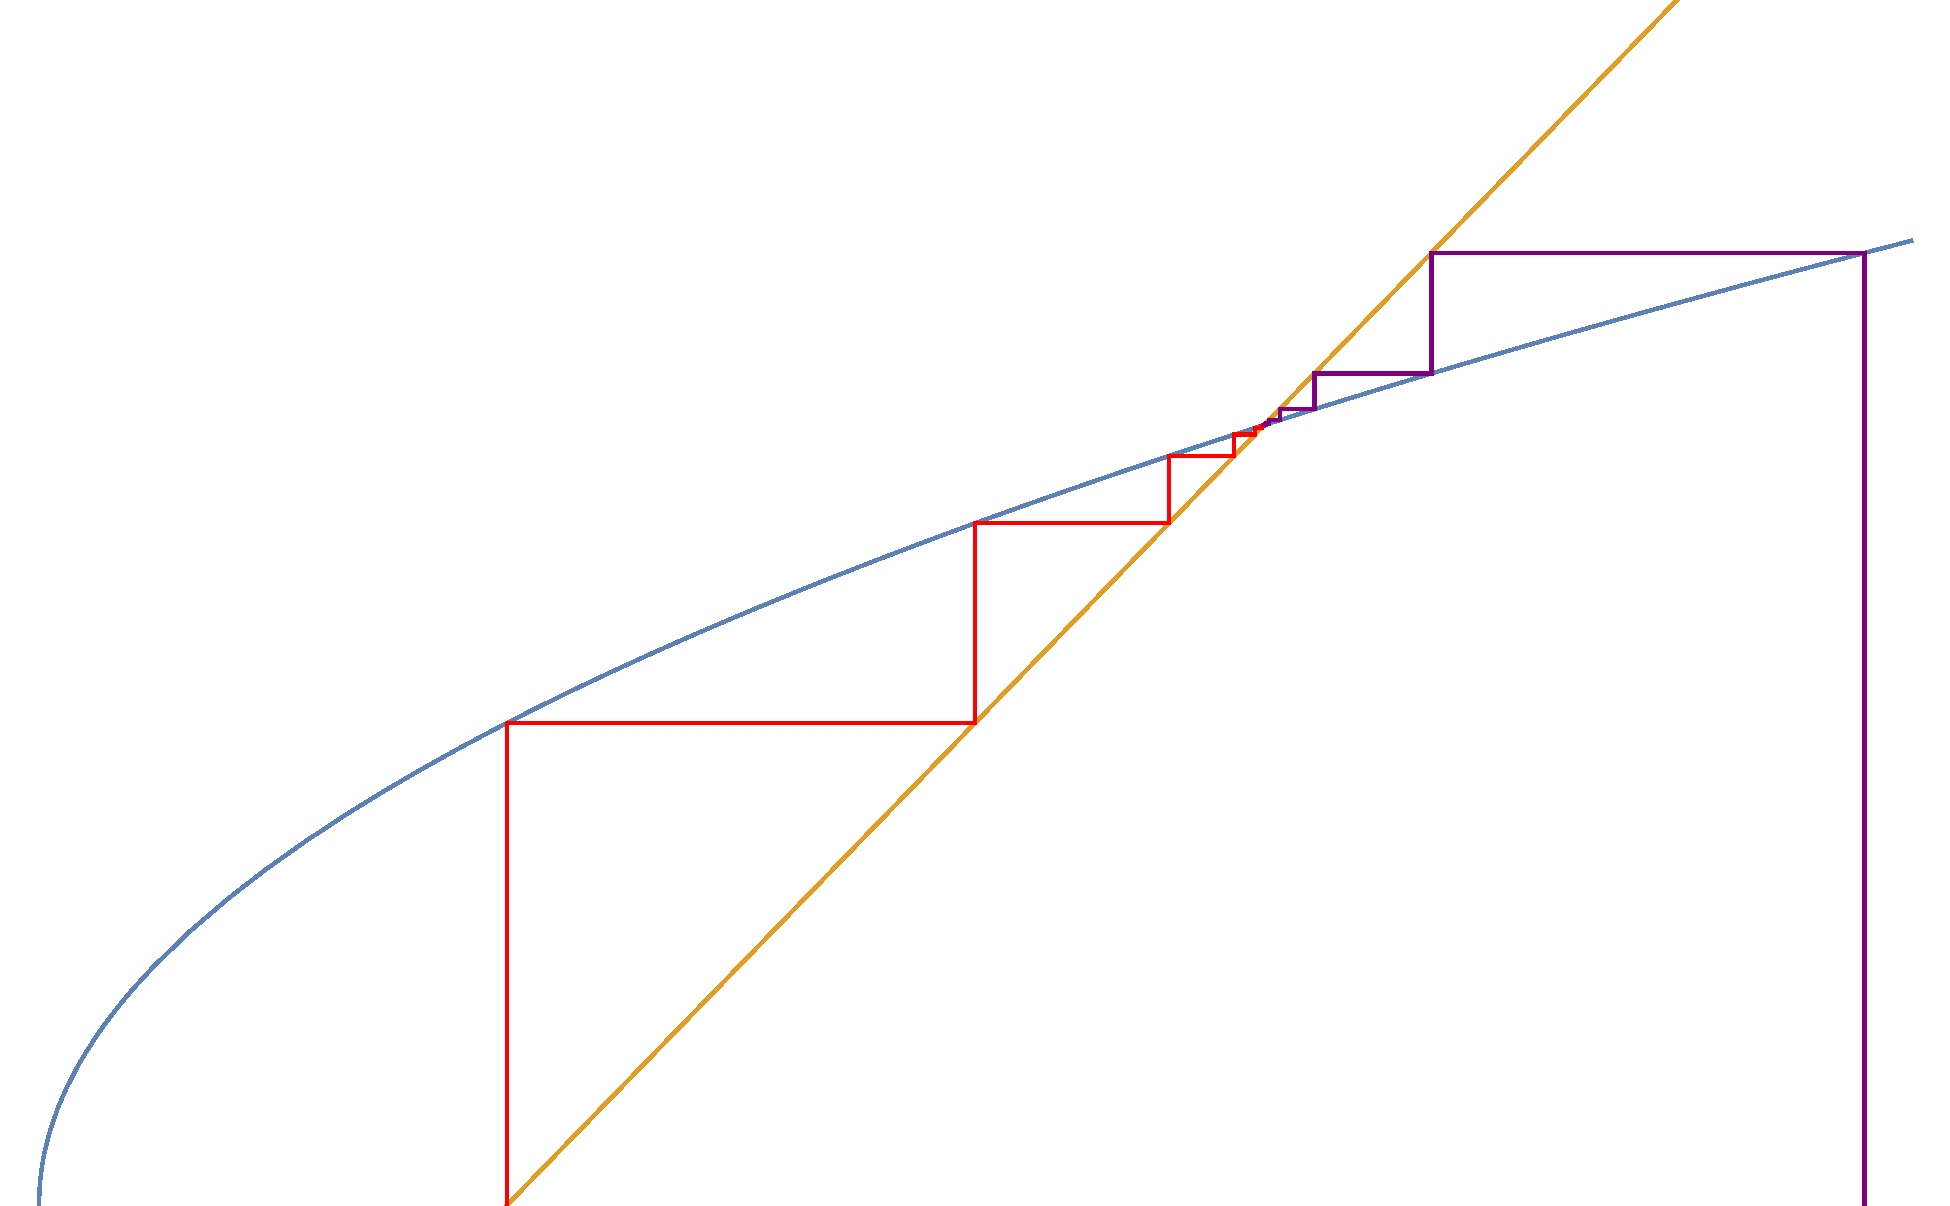
\includegraphics[scale=0.3]{../../Commun/Images/maths-cours-turtle-1.pdf}};
\draw[->] (-5,-3.06) -- (6,-3.06) node[below] {$x$};
\draw[->] (-2.38,-3.06) -- (-2.38,3.5) node[left] {$y$};
\node at (5.8,1.9) {$y=\sqrt{1+x}$};
\node at (4.15,3.05) {$y=x$};
\end{tikzpicture}
\end{center}
\begin{sol}
On commence par montrer que $(u_n)$ est bien définie en prouvant l'assertion $H_n$:"$u_n\geq 0$" par récurrence.

Recherche de points fixes : on tombe sur $(1+\sqrt{5})/2$.

On résout pour $x\geq 0$, $\sqrt{1+x}\geq x \Longleftrightarrow \ldots \Longleftrightarrow 0\leq x \leq (1+\sqrt{5})/2$.

\begin{itemize}
\item[$\bullet$] 1er cas : $\alpha> (1+\sqrt{5})/2$.

On démontre par récurrence $H_n : "(1+\sqrt{5})/2 \leq u_{n+1}\leq u_n".$
$(u_n)$ est donc décroissante minorée donc convergente et ça ne peut être que vers $(1+\sqrt{5})/2$.
\item[$\bullet$] 2ème cas : $\alpha < (1+\sqrt{5})/2$.
On démontre par récurrence $H_n : "(1+\sqrt{5})/2 \geq u_{n+1}\geq u_n".$
$(u_n)$ est donc croissante majorée donc convergente et ça ne peut être que vers $(1+\sqrt{5})/2$.
\end{itemize}
\end{sol}  
\exo Soit $\alpha\in\R$ et $(u_n)$ la suite définie par
  \[u_0\defeq\alpha \et \forall n\in\N \qsep u_{n+1}\defeq\frac{u_n^2+2}{3}.\]
 Étudier la limite éventuelle de la suite $(u_n)$.
% \begin{center}
% \begin{tikzpicture}[>=latex]
% \node at (0,0) {\includegraphics[scale=0.45]{../../Commun/Images/maths-cours-turtle-2.pdf}};
% \draw[->] (-7,-4.59) -- (5,-4.59) node[below] {$x$};
% \draw[->] (-5.435,-4.59) -- (-5.435,4.7) node[left] {$y$};
% \node at (1.8,4.6) {$y=\dfrac{x^2+2}{3}$};
% \node at (4.3,4.6) {$y=x$};
% \end{tikzpicture}
% \end{center}

\begin{sol}
$f$ est décroissante sur $\RM$ et croissante sur $\RP$.

On étudie les points fixes. On trouve $1$ et $2$.

On résout $f(x)\geq x$ : $S=[-\infty;1]\cup [2;+\infty]$.

\begin{itemize}
\item[$\bullet$] Si $\alpha \in [0;1]$. On souhaite montrer que $(u_n)$ est croissante et tend vers $1$. 
On commence par montrer par récurrence que $0\leq u_n\leq 1$. On en déduit que $(u_n)$ est croissante (de l'étude du signe de $f(x)-x$). Ainsi $(u_n)$ est croissante et majorée (par $1$) donc est convergente vers $\ell$. Puis un passage à la limite nous donne $\ell=\dfrac{\ell^2+2}{3}$ donc $\ell \in \set{1;2}$. Ainsi, $\ell=1$.


\item[$\bullet$] Si $\alpha \in [1;2[$, on montre successivement $1\leq u_n\leq 2$ par récurrence puis $u_{n+1}\leq u_n$. Ainsi $(u_n)$ est décroissante et minorée (par $1$) donc est convergente vers $\ell$. Puis un passage à la limite nous donne $\ell=\dfrac{\ell^2+2}{3}$ donc $\ell \in \set{1;2}$. Mais $u_n\leq u_0<0$ donc par passage à la limite, $\ell\leq u_0<0$  Ainsi, $\ell=1$.

\item[$\bullet$] Si $\alpha=2$, la suite est constante égale à $2$.

\item[$\bullet$] Si $\alpha \in ]2;+\infty[$. Par croissance de $f$ sur $]2;+\infty[$, on montre que $u_n>2 \forall n \in \N$. On montre ensuite que $u_{n+1}\geq u_n$. Ainsi, $u_n$ tend vers $\ell \in \R\cup\set{+\infty}$. Si $\ell$ est finie, un passage à la limite donne $\ell \in \set{1;2}$. Or $\forall n \in \N$, $2<u_0\leq u_n$ d'où $2<u_0\leq \ell$, ce qui est absurde. Donc $\ell=+\infty$.

\item[$\bullet$] Enfin si $\alpha \leq 0$, on remarque que $f(u_0)=f(|u_0|)$ par parité donc on est ramené au cas où $u_0\geq 0$. Ainsi,
\begin{itemize}
\item si $\alpha \in ]-2;2[$, $(u_n)$ tend vers $1$.
\item si $\alpha \in \set{-2;2}$, alors $(u_n)$ tend vers $2$.
\item si $\alpha \in ]-\infty;-2[\cup ]2;+\infty[$, alors $(u_n)$ tend vers $+\infty$.
\end{itemize}
\end{itemize}
\end{sol}
% \exo Soit $\alpha\in\R$ et $(u_n)$ la suite définie par $u_0\defeq\alpha$ et $\forall n\in\N \qsep u_{n+1}\defeq\cos(u_n)$. Étudier la convergence de la suite
%   $(u_n)$.
%   \begin{sol}
%   Montrer d'abord les lemmes suivants~: Si $I$ est stable par $f$ et que $f$
%   est croissante sur $I$, $(u_n)$ est monotone. Si $(u_{2n})$ et $(u_{2n+1})$
%   convergent vers la même limite alors $(u_n)$ est convergente. Les
%   points fixes de $f$ sont point fixe de $f\circ f$, mais la réciproque est
%   fausse.
%   Ensuite, on montrer que $\interf{0}{1}$ est stable par $\cos$ et que l'on
%   peut supposer que $\alpha\in\interf{0}{1}$. On montre que les suites
%   $(u_{2n})$ et $(u_{2n+1})$ sont monotones et donc convergent. Elles convergent
%   vers un point fixe de $cos\circ\cos$~: il n'y en a qu'un seul, le point fixe
%   de $\cos$.
%   \end{sol}
% \exo Soit $(u_n)$ la suite définie par
% \[u_0\defeq 1 \et \forall n\in\N\qsep u_{n+1}\defeq\frac{2u_n+2}{u_n+2}.\]
% \begin{questions}
% \question Montrer que la fonction $f$ définie sur $\RP$ par
%   \[\forall x\in\RP\qsep f(x)\defeq\frac{2x+2}{x+2}\]
%   admet un unique point fixe $\alpha$.
% \question Montrer que $f$ est contractante. En déduire que $u_n\tendvers{n}{+\infty}\alpha$.
% \end{questions}
\end{exos}

\begin{remarqueUnique}
\remarque Si $f$ est décroissante, on étudie les
      suites $(u_{2n})$ et $(u_{2n+1})$. Ces suites vérifient une relation de
      récurrence faisant intervenir $f\circ f$. On commence par étudier la suite $(u_{2n})$. Comme $f$ est décroissante, $f\circ f$ est croissante, et on est ramené au cas précédent. Puis, en remarquant que $u_{2n+1}=f(u_{2n})$, on en déduit la limite, si elle existe, de $(u_{2n+1})$. Si ces deux suites
      admettent la même limite $l\in\R$, alors $(u_n)$ converge vers $l$. Dans
      le cas contraire, la suite $(u_n)$ est divergente.
\end{remarqueUnique}


\begin{exoUnique}
\exo Étudier la suite $(u_n)$ définie par
\[u_0\defeq 0\et\forall n\in\N\qsep u_{n+1}\defeq 1-\frac{3}{4}u_n^2.\]
\begin{center}
\begin{tikzpicture}[>=latex]
\node at (0,0) {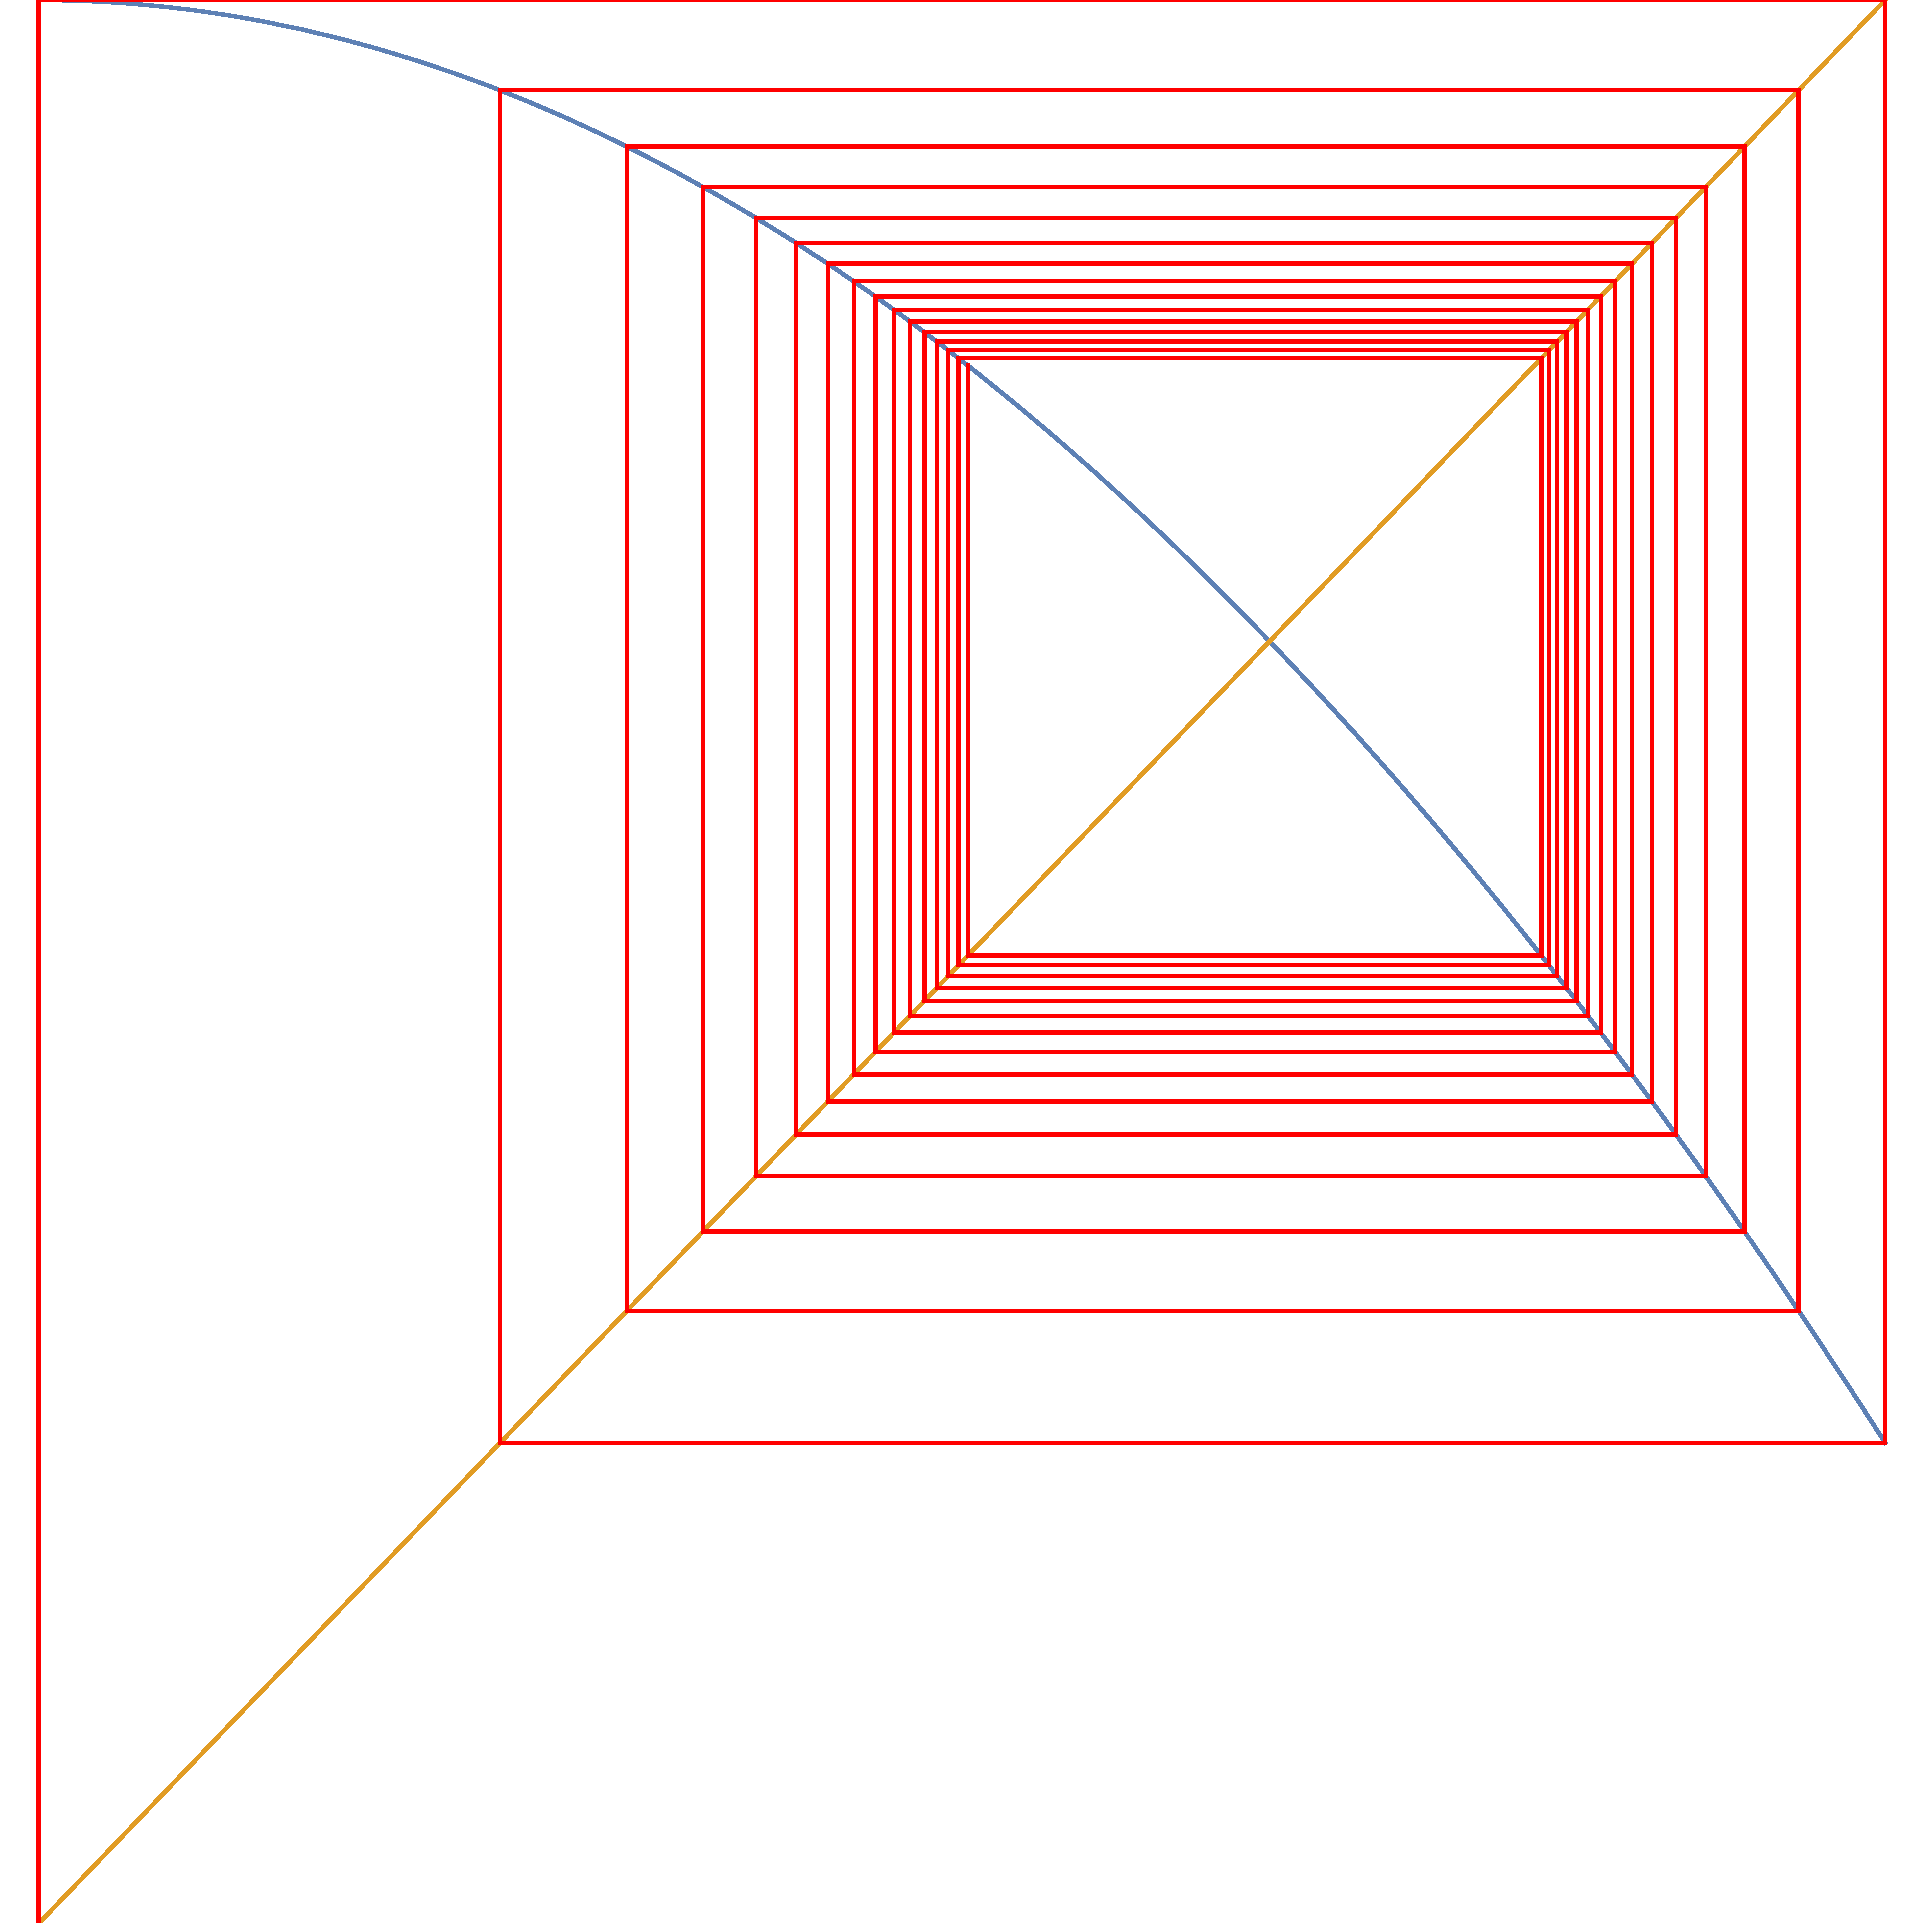
\includegraphics[scale=0.27]{../../Commun/Images/maths-cours-turtle-3.pdf}};
\draw[->] (-4.22,-4.4) -- (5.3,-4.4) node[below] {$x$};
\draw[->] (-4.22,-4.4) -- (-4.22,5.3) node[left] {$y$};
\node at (5.3,-2.15) {$y=1-\dfrac{3}{4}x^2$};
\node at (4.8,4.4) {$y=x$};
\end{tikzpicture}
\end{center}
\end{exoUnique}

\begin{sol}
Remarquons que 
\begin{itemize}
\item $f$ est décroissante sur $\RP$ et croissante sur $\RM$ donc $f\circ f$ est croissante.
\item Les points fixes de $f$ sont $-2$ et $2/3$.
\item ($f$ est paire.)
\end{itemize}
Nous allons donc étudier $(u_{2n})$ puis $(u_{2n+1})$.
\begin{itemize}
\item[$\bullet$] Déjà, $0\leq u_0\leq 2/3$ et si $0\leq u_{2n} \leq 2/3$ par croissance de $f\circ f$, on a $1/4=(f\circ f)(0)\leq (f\circ f)(u_{2n})=u_{2n+2} \leq (f\circ f)(2/3)=2/3$ donc par récurrence $0\leq u_{2n} \leq 2/3$ $\forall n \in \N$. 

De plus, $$(f\circ f)(x)-x=\frac{-1}{64}\p{27x^4-72x^2+64x-16}=\frac{-1}{64}(3x-2)(9x^3+6x^2-20x+8)$$ donc $$(f\circ f)(x)-x=\frac{-1}{64}(3x-2)(x+2)(9x^2-12x+4)=\frac{-1}{64}(3x-2)^3(x+2).$$
On peut alors dresser le tableau de signes de $(f\circ f)(x)-x$. Cela nous permet alors de dire que $(u_{2n})$ est croissante et majorée (par $2/3$) donc converge vers une limite $\ell$ qui par passage à la limite ne peut être que $2/3$.

\item[$\bullet$] $2/3\leq u_1 $ et par croissance de $f\circ f$, on déduit que $\forall n \in \N, 2/3\leq u_{2n+1}$. Avec le signe de $(f\circ f)(x)-x$ on peut voir que $(u_{2n+1})$ est décroissante et minorée (par $2/3$) donc converge vers une limite $\ell$ qui par passage à la limite ne peut être que $2/3$.

\end{itemize}

Pour conclure, $(u_{2n})$ et $(u_{2n+1})$ convergent vers une même limite donc $(u_n)$ est convergente (vers $2/3$).
\end{sol}

\subsection{Suites adjacentes}

\begin{definition}[utile=-3]
Soit $\p{u_n}$ et $\p{v_n}$ deux suites réelles. On dit que $\p{u_n}$ et
$\p{v_n}$ sont \emph{adjacentes} lorsque
\begin{itemize}
\item $\forall n\in\N \qsep u_n \leq v_n$,
\item $\p{u_n}$ est croissante et $\p{v_n}$ est décroissante,
\item $v_n-u_n \tendvers{n}{+\infty} 0$.
\end{itemize}
\end{definition}

\begin{remarqueUnique}
\remarque Si deux suites $(u_n)$ et $(v_n)$ vérifient les deux derniers points,
  alors elles vérifient le premier point. En théorie il est donc inutile de
  le vérifier, mais l'usage veut qu'on le fasse.
\end{remarqueUnique}

\begin{sol}
On va le montrer au travers de la prochaine preuve. On n'utilisera pas $(i)$ comme hypothèse, mais comme une conséquence de $(ii)$ et $(iii)$.
\end{sol}

\begin{proposition}[utile=-3]
Soit $\p{u_n}$ et $\p{v_n}$ deux suites adjacentes. Alors $\p{u_n}$ et $\p{v_n}$
convergent vers la même limite $l\in\R$. De plus
\[\forall n\in\N \qsep u_n \leq l \leq v_n.\]
\end{proposition}

\begin{preuve}
On suppose $u$ croissante et $v$ décroissante.
La suite $w=u-v$ est donc croissante et tend vers $0$. Donc $w_n\leq 0$. En effet, raisonnons par l'absurde. S'il existe un rang $N$ tel que $w_N>0$ par croissance, tous les rangs suivants sont $\geq w_N$ + passage à la limite.... Ainsi, $u_n\leq v_n\leq v_0$.
$u$ est croissante et majorée par $v_0$ donc converge vers $\ell$. $v=(v-u)+u$ converge donc vers $\ell$ aussi. 
\end{preuve}

\begin{exoUnique}
\exo Montrer que les suites $(u_n)$ et $(v_n)$ définies par
  \[\forall n\in\Ns \qsep u_n\defeq\sum_{k=1}^n \frac{1}{n+k} \et
    v_n\defeq\sum_{k=n}^{2n} \frac{1}{k}\]
  sont adjacentes. En utilisant une comparaison avec des intégrales, montrer
  qu'elles convergent vers $\ln 2$.
\end{exoUnique}

\begin{sol}
On a 
$$v_{n+1}-v_n=\frac{-3n-2}{n(2n+1)(2n+2)}\leq 0$$
donc $(v_n)$ est décroissante et $$u_{n+1}-u_n=\frac{1}{(2n+1)(2n+2)}\geq 0$$ donc $(u_n)$ est croissante. De plus, $v_n-u_n=\dfrac{1}{n}$.
Donc les suites sont adjacentes et convergent vers la même limite $\ell$.
En outre, $\forall k\geq 2$, $$\ln(k+1)-\ln(k)=\integ{k}{k+1}{\frac{1}{x}}{x}\leq \frac{1}{k} \leq \integ{k-1}{k}{\frac{1}{x}}{x}=\ln(k)-\ln(k-1)$$ donc $\forall n\geq 2$, on a en sommant de $n$ à $2n$ :
$$\ln(2n+1)-\ln(n)\leq v_n \leq \ln(2n)-\ln(n-1).$$
\end{sol}

\subsection{Théorème de \nom{Bolzano-Weierstrass}}

\begin{theoreme}[nom={Théorème de \nom{Bolzano-Weierstrass}}]
Toute suite bornée admet une sous-suite convergente.
\end{theoreme}

\begin{preuve}
\begin{itemize}
\item[$\bullet$] \underline{Cas réel (par dichotomie) :} Soit $u$ une suite réelle bornée. On peut fixer $K>0$ tel que $\forall n\in \N, u_n\in \interf{-K}{K}$. Posons $a_0=-K$, $b_0=K$ et $\varphi(0)=0$. On a bien $u_{\varphi(0)}\in \interf{a_0}{b_0}$.\\
Définissons \[E_0=\ens{n\in\N | u_n \in \interf{-K}{0}} \text{ et } E'_0=\ens{n\in\N | u_n \in \interf{0}{K}}.\] L'une au moins des deux parties est infinie, on choisit l'intervalle correspondant et on note $[a_1,b_1]$ cet intervalle. Comme l'ensemble choisi est infini, on peut en particulier fixer un élément $u_{\varphi(1)}$ dans $[a_1,b_1]$ tel que $\varphi(1)>\varphi(0)$.\\
Soit $p\in \N$. Supposons construit $\interf{a_p}{b_p} \subset\interf{a_{p-1}}{b_{p-1}}\subset\ldots\subset\interf{a_0}{b_0}$ et $\varphi(0)<\varphi(1)<\ldots<\varphi(p)$. Définissons \[E_p=\ens{n\in\N | u_n \in \interf{a_p}{\frac{a_p+b_p}{2}}} \text{ et } E'_p=\ens{n\in\N | u_n \in \interf{\frac{a_p+b_p}{2}}{b_p}}.\]
L'union des deux est infinie par construction donc l'un des deux est infini. On le choisit et on note $\interf{a_{p+1}}{b_{p+1}}$ l'intervalle correspondant. Comme l'ensemble choisi est infini, on peut en particulier fixer un élément $u_{\varphi(p+1)}$ dans $\interf{a_{p+1}}{b_{p+1}}$ tel que $\varphi(p+1)>\varphi(p)$.\\

On construit ainsi, par récurrence, une suite de segments de $\R$ décroissante au sens de l'inclusion et telle que $b_n-a_n=\dfrac{2K}{2^n}$ et telle que $\forall n\in \N$, $u_{\varphi(n)}\in \interf{a_n}{b_n}$.

D'après le théorème des segments emboités, $\displaystyle \bigcap_{n\in \N}\interf{a_n}{b_n}=\ens{\ell}$.

$\forall n\in \N$, comme $u_{\varphi(n)}$ et $\ell$ sont dans $\interf{a_n}{b_n}$, on a : $\abs{u_{\varphi(n)}-\ell}\leq \dfrac{2K}{2^n}$ d'où le résultat d'après le théorème des gendarmes.
\item[$\bullet$] \underline{Cas complexe :} Soit $u\in\C^\N$ bornée. Posons $x=\Re u$ et $y=\Im u$. Comme $u$ est bornée, $x$ l'est. D'après le cas réel, il existe une extraction $\varphi_1$ et un réel $\alpha$ tels que $x_{\varphi_1(n)}\tendvers{n}{+\infty}\alpha$.

La suite $(y_{\varphi_1(n)})_{n\in\N}$ est bornée. Il existe donc une extraction $\varphi_2$ et un réel $\beta$ tels que $y\circ \varphi_1 \circ \varphi_2=(y_{\varphi_1\circ\varphi_2(n)})_{n\in\N}$ converge vers $\beta$.
Posons $\varphi=\varphi_1\circ\varphi_2$. C'est une extraction. $x\circ\varphi$ est convergente comme suite extraite de $x\circ\varphi_1$ et $y\circ\varphi$ aussi.\\

Finalement, $u\circ \varphi$ est convergente.
\end{itemize}
\end{preuve}

\begin{exoUnique}
\exo Soit $x\in\R\setminus\Q$, $(p_n)$ une suite d'entiers relatifs et
  $(q_n)$ une suite d'entiers naturels non nuls tels que
  \[\frac{p_n}{q_n}\tendvers{n}{+\infty} x.\]
  Montrer que $q_n\tendvers{n}{+\infty}+\infty$.
\end{exoUnique}
\begin{sol}
Raisonnons par l'absurde. Cela signifie qu'il existe $m\in \R$ tel que $\forall N \in \N, \exists n\geq N$ tel que $q_n < m$.
Fixons un tel $m$ et construisons une extractrice $\phi$ telle que $\forall n \in \N$, $1\leq q_{\phi(n)}\leq m$.
\begin{itemize}
\item[$\bullet$] On pose $N=0$. Il existe $n\geq 0$ tel que $q_n<m$. On pose $n=\phi(0)$.
\item[$\bullet$] Soit $k\in \N$. On suppose construit $\phi(0)< \ldots< \phi(k)$ tels que $1\leq u_{\phi(k)}\leq m$.
On pose $N=\phi(k)+1$. Alors, il existe $n\geq N$ tel que $q_n<m$. On pose $\phi(k+1)=n$...
\end{itemize}
La suite $(q_{\phi(n)})$ est donc bien construite et bornée. Elle admet donc une sous-suite convergente, c'est-à-dire qu'il existe $\psi$ telle que $(q_{\phi(\psi(n))})$ converge vers $\ell \in \R$. Comme il s'agit d'une suite d'entiers convergentes, elle est constante apcr et donc $\ell \in \Ns$. Mais alors $\displaystyle p_{\phi(\psi(n))}=\frac{p_{\phi(\psi(n))}}{q_{\phi(\psi(n))}}q_{\phi(\psi(n))} \tendvers{n}{+\infty}{\ell x}=\ell'$ et pour les mêmes raisons $\ell' \in \Z$.
Ainsi, $\displaystyle \frac{p_{\phi(\psi(n))}}{q_{\phi(\psi(n))}} \tendvers{n}{+\infty} \frac{\ell'}{\ell} \in \Q$. Donc $x\in \Q$ par unicité de la limite, ce qui fournit une contradiction.
\end{sol}
%END_BOOK

\end{document}


